\documentclass[a4paper,10pt]{article}
\usepackage[utf8x]{inputenc}
\usepackage[czech]{babel}

\usepackage{amsthm}
\usepackage{amsmath}
\usepackage{amsfonts}
\usepackage{mathtools}

%% číslovaný cases
\usepackage[subnum]{cases}

%% colspan a rowspan v tabulkách
\usepackage{multirow}

%%  http://tex.stackexchange.com/a/361157
\usepackage{showlabels}

%% subfigures, https://en.wikibooks.org/wiki/LaTeX/Floats,_Figures_and_Captions#Subfloats
\usepackage{subcaption}

%% číslování řádků, https://texblog.org/2012/02/08/adding-line-numbers-to-documents/
\usepackage{lineno}

%Definice, věta, důkaz!
\newtheorem{definition}{Definice}
\newtheorem{theorem}{Věta}
\newtheorem*{notation*}{Značení}
\newtheorem{note}{Poznámka}
\newtheorem{example}{Příklad}


\numberwithin{definition}{section}
\numberwithin{theorem}{section}
%\numberwithin{notation}{section}
\numberwithin{note}{section}
\numberwithin{example}{section}


%Ostatní makra
\newcommand{\TODO}[1]{ \textit{\small(zde bude doplněno: #1)} }	
\newcommand{\RLY}{?? }

\newcommand{\lattL}{\mathbb{L}}
\newcommand{\fsubsets}[1]{\mathcal{F}(#1)}

\newcommand{\term}[1]{\textit{#1}}
\newcommand{\str}[1]{{\ttfamily#1}}
\newcommand{\regex}[1]{{\ttfamily#1}}

\newcommand{\impl}[2]{{\ttfamily#1/}{\ttfamily test/data/}{\ttfamily#2}}

% Speciální nastavení

% vycentrované floating objekty
% http://tex.stackexchange.com/questions/2651/should-i-use-center-or-centering-for-figures-and-tables
\makeatletter
\g@addto@macro\@floatboxreset\centering
\makeatother

\linenumbers
\modulolinenumbers[10]


%opening
\title{Aplikace fuzzy a pravděpodobnostních automatů}
\author{Martin Jašek}
\date{12. září 2016 --- ??}

\begin{document}

\maketitle
\tableofcontents
\newpage

%%%%%%%%%%%%%%%%%%%%%%%%%%%%%%%%%%%%%%%%%%%%%%%%%%%%%%%%%%%%%%%%%%%%%%%%%%%%%%%
\section{Definice a značení}
Tato kapitola zatím poslouží jako \uv{skladiště} pro definice a zavedení značení pro ostatní kapitoly.
%V této kapitole budou rozebrány různé definice fuzzy automatů, jejich vztahy (který je speciálním případem kterého apodob.), vlastnosti... Aktuálně však složí jen jako \uv{skladiště} definic, aby bylo na co se odkazovat v ostatních kapitolách.

\subsubsection*{Abecedy, řetězce, jazyky}
Abecedy budou značeny standardně, tedy velkými řeckými písmeny (typicky $\Sigma$). Řetězce pak malými písmeny ($\omega, \alpha, \dots$). Jazyky velkými kaligrafickými písmeny. Jazyk přijímaný automatem $A$ bude značen $\mathcal{L}(A)$.

\subsubsection*{Fuzzy teorie}
Fuzzy množiny a relace budou po vzoru \cite{AstGonMenGar-FuzzAutEpsMovCmpFuzzMeasBtwStrs} nejčastěji malými řeckými písmeny (obdobně jako jejich členské (angl. \uv{membership}) funkce). Množinu všech fuzzy podmnožin množiny $S$ budeme značit $\fsubsets{S}$.

\subsubsection*{Deterministický bivalentní automat}
\TODO{zdroj: Eilenberg S.: Automata, Languages and Machines, Vol. A, Academic Press, New York, 1974. Pokud ji někde seženu (odkazuje se na ni Bel v \cite{Bel-FuzRelSyss}}

\TODO{co citování definic? půlku jsem si vymyslel ...}

\begin{definition}
 Konečný deterministický (bivalentní) automat je pětice $A = ( Q, \Sigma, \delta, q_0, F )$, kde $Q$ je konečná množina stavů, $\Sigma$ je vstupní abeceda, $\delta: Q \times \Sigma \rightarrow Q$ je přechodová funkce, $q_0 \in Q$ je počátační stav a $F \subseteq Q$ je množina koncových stavů.
\end{definition}


\subsubsection*{Nedeterministický bivalentní automat}
\TODO{Značení převzato z FJAA, dohledat zdroj}
\begin{definition}
 Konečný nedeterministický (bivalentní) automat je pětice $A = ( Q, \Sigma, \delta, I, F )$, kde $Q$ je konečná množina stavů, $\Sigma$ je vstupní abeceda, $\delta: Q \times \Sigma \rightarrow 2^Q$ je přechodová funkce, $I \subseteq Q$ je množina počátačních stavů a $F \subseteq Q$ je množina koncových stavů.
\end{definition}


\subsubsection*{Základní definice nedeterministického fuzzy automatu}
Značení je převzato z \cite{AstGonMenGar-FuzzAutEpsMovCmpFuzzMeasBtwStrs} a lehce upraveno.

\begin{definition}[Nedeterministický fuzzy automat]\label{def-ZaklDefNedFuzzAut}
 Nedeterministický fuzzy automat $A$ je pětice $(Q, \Sigma, \mu, \sigma, \eta)$, kde $Q$ je konečná množina stavů, $\Sigma$ je abeceda, $\mu$ je fuzzy přechodová funkce (fuzzy relace $Q \times \Sigma \times Q \rightarrow [0, 1]$) a $\sigma$ a $\eta$ jsou po řadě fuzzy množiny nad $Q$ počátačních, resp. koncových stavů.
\end{definition}

\begin{definition}[Fuzzy stav]\label{def-FuzzStav}
 Mějme nedeterministický fuzzy automat $A$. Pak jako fuzzy stav označujeme fuzzy podmnožinu jeho stavů, tj. $V \in \fsubsets{Q}$.
\end{definition}

\begin{definition}[Aplikace fuzzy relace na fuzzy stav]
 Mějme nedeterministický fuzzy automat $A$ a fuzzy symbol $V$. Pak aplikací binární fuzzy relace $R: Q \times Q \rightarrow [0, 1]$ na fuzzy stav $V$ obdržíme fuzzy symbol $V \circ R$ splňující pro každé $p \in Q$: $(V \circ R )(p) = \max_{q \in Q} (V(q) \otimes R(q, p))$.
\end{definition}

\begin{definition}[Přechodová funkce fuzzy stavů]\label{def-PreFunFuzzStav}
 Mějme nedeterministický fuzzy automat $A$. Pak přechodová funkce fuzzy stavů je fuzzy relace $\widehat{\mu}: \fsubsets{F} \times \Sigma \rightarrow \fsubsets{F}$ taková, že pro každý fuzzy stav $V \in \fsubsets{Q}$ a symbol $x \in \Sigma$ je $\widehat{\mu}(V, x) = V \circ \mu[x]$.
\end{definition}

\begin{note}
 Označení $\mu[x]$ je fuzzy relace, pro kterou platí: $\mu[x](p, q) = \mu(p, x, q)$ pro všechna $x \in \Sigma$ a $p, q \in Q$.
\end{note}

\begin{definition}[Rozšířená přechodová funkce]\label{def-PreFunFuzzStav}
 Mějme nedeterministický fuzzy automat $A$. Pak rozšířená přechodová funkce (fuzzy stavů) je fuzzy relace $\mu^*: \fsubsets{F} \times \Sigma^* \rightarrow \fsubsets{F}$ (\TODO{co je to $F$? Nemá to být $Q$?!}) daná následujícím předpisem:
 \begin{enumerate}
  \item $\mu^*(V, \epsilon) = V$ pro všechna $V \in \fsubsets{Q}$
  \item $\mu^*(V, \alpha x) = \widehat{\mu}(\mu^*(V, \alpha), x)$ pro všechna $V \in \fsubsets{Q}, \alpha \in \Sigma^*, x \in \Sigma$
 \end{enumerate}
\end{definition}

\begin{definition}[Řetězec přijímaný automatem]\label{def-RetPriAut}
 Mějme nedeterministický fuzzy automat $A$. Pak řětězec $\alpha \in \Sigma^*$ je automatem $A$ přijat ve stupni
 $$
  A(\alpha) = \max_{q \in Q} (\mu^*(\sigma, \alpha)(q) \otimes \eta(q))
 $$
 \TODO{ověřit, dohledat, ozdrojovat}
\end{definition}

\begin{definition}[Jazyk rozpoznávaný automatem]\label{def-JazRozpAut}
 Mějme nedeterministický fuzzy automat $A$. Pak fuzzy množinu $\mathcal{L}(A)(\alpha) = A(\alpha)$ nad univerzem $\Sigma^*$ nazýváme fuzzy jazyk rozpoznávaný automatem $A$.

 \TODO{ověřit, dohledat, ozdrojovat}
\end{definition}

\subsubsection*{Nedeterministický fuzzy automat s $\epsilon$ přechody}

\begin{definition}[Nedeterministický fuzzy automat s $\epsilon$ přechody]\label{def-NedFuzzAutEpsPre}
\TODO{dohledat přesně, zkontrolovat a ozdrojovat}
 Nedeterministický fuzzy automat $A$ je pětice $(Q, \Sigma, \mu, \sigma, \eta)$, kde $Q$ je konečná množina stavů, $\Sigma$ je abeceda, $\mu$ je fuzzy přechodová funkce (fuzzy relace $Q \times (\Sigma \cup \{ \epsilon \}) \times Q \rightarrow [0, 1]$) a $\sigma$ a $\eta$ jsou po řadě fuzzy množiny nad $Q$ počátačních, resp. koncových stavů.
\end{definition}

\TODO{Tady by asi bylo vhodné rozebrat $\epsilon$-uzávěry}

\subsubsection*{Reprezentace fuzzy automatu}
\TODO{dohledat zdroje}

\TODO{Značení fuzzy množiny $\sigma = \{ x/0.5 \}$ vs. $\sigma(x) = 0.5$} 

Přechodový diagram: Notace s lomítky např. zde: \cite{GonGar-FuzzLangInfRanAccGuzzAutPumLemDetProc}.

Tabulka: stav $\times$ symbol nebo stav $\times$ stav \cite{DooKre-NewDirFuzzAut}?

\subsubsection*{Konstrukce fuzzy automatu z konečného automatu}
V praxi se často setkáme z problémem, kdy máme k dispozici konečný bivalentní automat avšak my potřebujeme pro naši práci fuzzy automat. Je tedy třeba zkonstruovat takový fuzzy automat, který rozpoznává odpovídající jazyk odpovídající jazyku rozpoznávaném naším bivalentním automatem. 

Důležité je zmínit, že nelze zkonstruovat fuzzy automat, rozpoznávající stejný jazyk neboť fuzzy automat rozpoznává fuzzy jazyk, zatímco bivaletní automat klasický \uv{bivalentní} jazyk. Můžeme však sestavit automat takový, který přijímá řetězce ve stupni $0$ nebo $1$ podle toho, jestli je přijímal bivaletní automat.

Formálně řečeno, pro konečný (nedeterministický) bivalentní automat $A$ budeme konstruovat nedeterministický fuzzy automat $A'$ takový, že bude pro všechna $x \in \Sigma^*$ splněna následující rovnost:
$$
 \mathcal{L}(A')(\omega) = 
  \begin{cases}
   1 & \text{ pokud } \omega \in \mathcal{L}(A) \\
   0 & \text{ pokud } \omega \notin \mathcal{L}(A)
  \end{cases}
$$

\begin{note}
 Postup budeme provádět pro nedeterministické automaty. To jednak proto, že nedeterministické automaty jsou obecnější, než deterministické, a navíc, protože jsou v praxi využívány častěji. \TODO{ozdrojovat, klidně někde, kde rozebírám determinizmus vs. nedeterminizmus}
\end{note}

Nyní se podíváme na to, jak výsledný fuzzy automat bude vypadat. Abeceda i množina stavů automatu zůstanou zachovány, lišit se tedy bude pouze množina počátečních a koncových stavů a přechodová funkce. \TODO{fuzzy subset $I$, $F$ a $\delta$? nebo tak něco, z teorie fuzzy množin?}

\begin{definition}[Fuzzy automat bivalentního automatu] \label{def-FuzzAutBivAut}
  Mějme řetězec konečný nedeterministický automatu $A = ( Q, \Sigma, \delta, I, F )$. Pak nedetermintistický fuzzy automat přijímájící korespondující jazyk je automat $A' = ( Q, \Sigma, \mu, \sigma, \epsilon )$ kde pro všechna $q_i, q_j \in Q$ a $x \in \Sigma$:
  \begin{itemize}
   \item $\sigma(q_i) =
    \begin{cases}
     1 & \text{ pokud } q_i \in I \\
     0 & \text{ pokud } q_i \notin I
    \end{cases}$
    
   \item $\eta(q_i) =
    \begin{cases}
     1 & \text{ pokud } q_i \in F \\
     0 & \text{ pokud } q_i \notin F
    \end{cases}$
    
    \item $\mu(q_i, x, q_j) = 
     \begin{cases}
      1 & \text{ pokud } q_j \in \delta(q_i, x) \\
      0 & \text{ pokud } q_j \notin \delta(q_i, x)
     \end{cases}$
  \end{itemize}
\end{definition}

\TODO{rozebrat, jestli tento automat skutečně dělá to, co má? Asi by to chtělo}

\TODO{vymyslet nějaký fakt pěkný příklad}

%%%%%%%%%%%%%%%%%%%%%%%%%%%%%%%%%%%%%%%%%%%%%%%%%%%%%%%%%%%%%%%%%%%%%%%%%%%%%%%
%%%%%%%%%%%%%%%%%%%%%%%%%%%%%%%%%%%%%%%%%%%%%%%%%%%%%%%%%%%%%%%%%%%%%%%%%%%%%%%

\section{Fuzzy automaty, gramatiky a jazyky}
\TODO{nějak to uvést. Budou pojmy jako regulérní jazyk a gramatika popsány v nějaké předchozí kapitole?}

\TODO{pojem \uv{Lattice language}}

\TODO{značení: \uv{Fuzzy množina $\phi$} vs. \uv{$L$-množina $\phi: X \rightarrow L$}; \uv{fuzzy podmnožina} vs. \uv{fuzzy množina nad}}
% asi k ničemu: DooKre-NewDirFuzzAut \cite{DooKre-NewDirFuzzAut}, 
% asi zbytečně vědátorské, nám stačí jazyk nad [0,1]: PalYau-FracFuzzGramAppPatRec \cite{PalYau-FracFuzzGramAppPatRec}?,
% okay: GonGar-FuzzLangInfRanAccGuzzAutPumLemDetProc \cite{GonGar-FuzzLangInfRanAccGuzzAutPumLemDetProc},
% fjuuh: StaCir-ConsFuzzAutFuzzRegExp \cite{StaCir-ConsFuzzAutFuzzRegExp},
% blbost, nic tam není: RamGir-CharFuzzRegLang \cite{RamGir-CharFuzzRegLang},


\subsection{Jazyk rozpoznávaný fuzzy automatem}
Věta 6.3 \cite{LiPed-FuzzFinAutFuzzRegExMembValLattOrdMon} (pro lattice monoid, není to někde jen pro $[0,1]$?).

Dle definice 4 \cite{GonGar-FuzzLangInfRanAccGuzzAutPumLemDetProc} je fuzzy regulární jazyk fuzzy podmnožina bivalentního.

Automat s bivalentní $\mu$ and $\eta$ (a fuzzy $\sigma$) taky rozpoznává fuzzy regulérní jazyk \cite{PalYau-FracFuzzGramAppPatRec}. Neřešil něco takového i Bel? Jinak řečeno, support konečný automat \cite{GonGar-FuzzLangInfRanAccGuzzAutPumLemDetProc}.

\subsection{Fuzzy a bivalentní regulérní jazyky}
Univerzum fuzzy jazyka je regulérní jazyk, pozorování 6.1 \cite{LiPed-FuzzFinAutFuzzRegExMembValLattOrdMon}.

Stejně tak, zaříznutý jazyk ($a$-řez jazyka) je také regulérní, věta 2.2 \cite{PalYau-FracFuzzGramAppPatRec}. 

Pumping lemma pro fuzzy regulérní jazyky, lemma 4-7 pro různé typy automatů \cite{GonGar-FuzzLangInfRanAccGuzzAutPumLemDetProc}.

Uzávěrové vlastnosti fuzzy regulérních jazyků, např. \cite{PalYau-FracFuzzGramAppPatRec}.
\subsection{Fuzzy regulární výrazy}
LiPed-FuzzFinAutFuzzRegExMembValLattOrdMon, definice 5.1, 5.2 (+ opsat důkaz, že $[0, 1]$ je lattice monoid) \cite{LiPed-FuzzFinAutFuzzRegExMembValLattOrdMon}.

Algoritmus převodu reg na aut, \cite{StaCir-ConsFuzzAutFuzzRegExp}. Ale zdá se mi to až moc složité.

%%%%%%%%%%%%%%%%%%%%%%%%%%%%%%%%%%%%%%%%%%%%%%%%%%%%%%%%%%%%%%%%%%%%%%%%%%%%%%%
%%%%%%%%%%%%%%%%%%%%%%%%%%%%%%%%%%%%%%%%%%%%%%%%%%%%%%%%%%%%%%%%%%%%%%%%%%%%%%%



%%%%%%%%%%%%%%%%%%%%%%%%%%%%%%%%%%%%%%%%%%%%%%%%%%%%%%%%%%%%%%%%%%%%%%%%%%%%%%%
%%%%%%%%%%%%%%%%%%%%%%%%%%%%%%%%%%%%%%%%%%%%%%%%%%%%%%%%%%%%%%%%%%%%%%%%%%%%%%%
\section{Rozpoznávání textových vzorů}

Rozpoznávání vzorů obecně je jednou z nejvýznamějších aplikací informatiky. V běžném životě se často setkáváme se situacemi, kdy je třeba v datech najít výskyt učitého vzoru, popř. jeho další vlastnosti. Případně určit podobnost ke vzoru, nebo nejpodobnější vzor.

Typickým příkladem je např. detekce obličeje na fotografii, tedy rozpoznávání vzorů v obrazových datech. Vzory je však možné rozpoznávat v téměř jakýchkoliv datech, například textech, zvukových záznamech či výsedcích měření nebo pozorování.

Z pohledu teoretické informatiky je však základem vyhledávání vzorů v textových datech. Textová data, tedy řetězce, mají jednoduchou strukturu a lze s nimi snadno manipulovat. Na druhou stranu, jsou schopna reprezentovat nebo kódovat široké spektrum dat. Právě z tohoto důvodu je studium rozpoznávání textových vzorů klíčové pro zpracovávání jakýchkoliv dalších typů dat.

\begin{note}
 Pokud nebude uvedeno jinak, pojem \uv{rozpoznávání textových vzorů} bude v této kapitole zkracován jen na \uv{rozpoznávání vzorů}.
\end{note}

%%%%%%%%%%%%%%%%%%%%%%%%%%%%%%%%%%%%%%%%%%%%%%%%%%%%%%%%%%%%%%%%%%%%%%%%%%%%%%%
\subsection{Formální zavedení problému}
Stejně tak, jak se mohou různit aplikace rozpoznávání vzorů, i samotný pojem \uv{rozpoznávání vzorů} bývá chápan různě. V nejzákladnější podobě se jedná o problém určení, zda-li pozorovaný řetězec odpovídá předem stanovenému vzoru. Vzorem bývá obvykle také řetězec, ale může jím být například regulérní výraz. Také - může nás zajímat buď exaktní shoda pozorovaného řetězce se vzorem, nebo jen nějaká forma podobnosti. 

V rozšířeném smyslu může být problém chápán jako klasifikace. Tedy, určení třídy, do které by měl pozorovaný řetězec spadat, typicky na základě podobnosti s vybrannými reprezentanty jednotlivých tříd. 

V této kapitole se však budeme zabývat pouze určováním podobnosti vzorového a pozorovaného řetězce. U každé instance problému budeme znát abecedu se kterou pracujeme a také vzor. Vzorem bude libovolný řetězec nad touto abecedou. Řešením tohoto problému pro nějaký, tzv. pozorovaný, vstupní řetězec bude úroveň podobnosti tohoto řetězce s vzorovým. Jako podobnost zde budeme uvažovat reálné číslo z intervalu $[0, 1]$, kde $0$ znamená úplnou rozdílnost a $1$ úplnou shodu. 

\begin{note}
 Vzorový řetězec budeme v této kapitole vždy značit $\omega$, pozorovaný pak $\alpha$.
\end{note}

Nyní máme zadefinován problém samotný, nicméně je třeba zdůraznit, že v jeho definici se používá vágní pojem \uv{podobnost řetězců}. Podobnost řetězců je totiž pojem, který souvisí s konkrétní instancí problému a nelze jej nějak přesně, ale současně dostatečně obecně popsat. Jedinné, co o podobnosti řetězců můžeme říct, je, že čím vyšší toto číslo je, tím by si měly být řetězce podobnější.

Například, budeme-li porovnávat vstup zadaný z klávesnice počítače oproti nějakému vzoru, je možné, že uživatel udělá překlep. V takovém případě bude vzorovému řetězci určitě více podobný řetězec obsahující dva překlepy (záměna symbolu za některý sousedící na klávesnici) než jiný, který se sice bude lišit jen v jednom symbolu, ale to takovém, který je na opačné straně klávesnice.

Obdobně, pokud budeme pracovat s abecedou malých a velkých písmen (majuskule a minuskule). Uvažujme vzorový řetězec \str{hello}. Řetězec \str{HELLO} se s ním neshoduje v ani jednom symbolu, ale přesto jejich podobnost může být blízká jedné.

% \begin{definition}[Problém rozpoznávání vzorů]
%   Mějme konečnou abecedu $\Sigma$ a řetězce $\omega, \alpha \in \Sigma^*$ nad touto abecedou. Řetězec $\omega$ nazývejme \term{vzor}, řetězec $\alpha$ pak \term{pozorovaný řetězec}. Problém rozpoznávání vzorů je problém určení podobnosti řetězce $\alpha$ od řetězce $\omega$. Pokud nebude uvedeno jinak, podobnost uvažijeme jako reálné číslo z intervalu $[0, 1]$.
% \end{definition}

%%%%%%%%%%%%%%%%%%%%%%%%%%%%%%%%%%%%%%%%%%%%%%%%%%%%%%%%%%%%%%%%%%%%%%%%%%%%%%%
\subsection{Motivace k použití fuzzy automatů}
Klasická teorie automatů vznikla jako nástroj pro zpracování textových řetězců. Z tohoto důvodu je rozpoznávání textových vzorů jejím základním výsledkem. Automaty obecně jsou nástroje sloužící pro rozhodování, zda-li řetězec odpovídá vzoru automatem reprezentovaném. Použití pro rozpoznávání řetězcového vzoru tak bude jen speciálním případem jejich užití.

V předchozí podkapitole jsme si stanovili, že řešením našeho problému je číslo z intervalu $[0,1]$. Z tohoto důvodu nebude možné využít klasické bivalentní automaty. Fuzzy automaty pracují se stupněm pravdivosti, který by mohl s hodnotou podobnosti řetězců korespondovat. Navíc, v praxi se často setkáme s texty, které jsou nepřesné a nedokonalé. Fuzzy přístup by nám tak mohl pomoci na tyto nepřesnosti adekvátně reagovat.

\TODO{a co pravděpodobnostní?} \TODO{Protože například: \uv{pozorovaný řetězec se se vzorovým shoduje ve stupni $x$} ale \uv{je pravděpodobnost $y$, že uživatel zadal požadovaný řetězec}}
%%%%%%%%%%%%%%%%%%%%%%%%%%%%%%%%%%%%%%%%%%%%%%%%%%%%%%%%%%%%%%%%%%%%%%%%%%%%%%%
\subsection{Automat rozpoznávající $\omega$}
Klíčovým pro rozpoznávání vzorů (chceme-li využívat fuzzy automaty) je bivalentní automat rozpoznávající vzorový řetězec. Tedy automat takový, který přijímá jedinný řetězec $\omega$ a všechny ostatní zamítá. Nyní si takovýto automat zkonstruujeme.

Uvažujme, že máme k dispozici vzorový řetězec $\omega$ nad abecedou $\Sigma$. Označme $\mathcal{L}(\omega)$ jako jednoprvkový jazyk obsahující pouze řetězec $\omega$. Vzhledem k tomu, že jazyk $\mathcal{L}(\omega)$ je konečný, je také regulérní a existuje tak konečný deterministický automat, který jej rozpoznává.

Automat bude v každém kroku konzumovat symboly ze vstupního řetězce a porovnávat je se symboly vzorového řetězce na odpovídajících pozicích. Pokud dojde ke shodě na všech pozicích, automat dojde do koncového stavu a sledovaný řetězec přijme. Pokud se symboly shodovat nebudou, automat nebude mít definován žádný odpovídající přechod, kterým by pokračoval ve výpočtu, a řetězec tak zamítne. 

Takovýto automat označme jako \term{automat rozpoznávající} $\omega$.
\begin{definition}[Automat rozpoznávající $\omega$ (deterministický)]
  Mějme řetězec $\omega$ délky $n$ nad abecedou $\Sigma$. Automat rozpoznávající $\omega$ je pak konečný automat $A(\omega) = ( Q, \Sigma, \delta, q_0, F )$ takový, že jeho množina stavů $Q$ se sestává z právě $n$ stavů $q_0, \dots, q_n$, $q_0$ je počáteční stav, $F = \{ q_n \}$ množina koncových stavů a $\delta$ je přechodová funkce definována pro všechna $0 \leq k < n$ následovně:
  $$
    \delta(q_{k}, a_k) = q_{k+1} \text{ kde $a_k$ je $k$-tý symbol řetězce $\omega$}
  $$
\end{definition}

Tato definice automatu je vcelku intuitivní. K stejnému výsledku bychom došli, pokud bychom automat zkonstruovali konverzí gramatiky nebo regulérního výrazu. 

\begin{example}
 Příklad automatu rozpoznávající řetězec $\omega = $ \str{hello} se nachází na obrázku \ref{diag-AutRozpHell}.  

  \begin{figure}
    \includegraphics{diags0}
    \caption{Automat rozpoznávající \str{hello}} \label{diag-AutRozpHell}
  \end{figure}
\end{example}

My však budeme potřebovat fuzzy automat rozpoznávající $\omega$. To znamená, že musíme nejdříve automat z předchozí definice převést na nedeterministický a poté dle definice \ref{def-FuzzAutBivAut} k němu zkonstruovat odpovídající fuzzy automat.

\begin{definition}[Automat rozpoznávající $\omega$ (nedeterministický)] \label{def-AutRozpOme}
  Mějme řetězec $\omega$ nad abecedou $\Sigma$ z předchozí definice. Nedeterministický automat rozpoznávající $\omega$ je pak konečný automat $A'(\omega) = ( Q, \Sigma, \delta, I, F )$ takový, že jeho množina stavů $Q$ je stejná jako v předchozí definici, dále $I = \{ q_0 \}$ je množina počátečních a $F = \{ q_n \}$ množina koncových stavů a $\delta$ je přechodová funkce definována pro všechna $0 \leq k < n$ následovně:
  $$
  \delta(q_{k}, a_k) = 
  \begin{cases}
      \{ q_{k+1} \}	&\text{pokud je $a_k$ $k$-tý symbol řetězce $\omega$} \\
      \emptyset	&\text{jinak}
  \end{cases}
  $$
\end{definition}

%TODO: Ekvivalentní definice je zavedena v \cite[str. 2]{AstGariGonVillFar-ApprStrMatUsiDefFuzzAutLearExpr}.
Následuje vytvoření fuzzy automatu.

\begin{definition}[Fuzzy automat rozpoznávající $\omega$] \label{def-FuzzAutRozpOme}
  Mějme řetězec $\omega$ nad abecedou $\Sigma$ délky $n$. Fuzzy automat rozpoznávající $\omega$ je pak automat $A''(\omega)$ vytvořený z nedeterministického automatu rozpoznávající $\omega$ (definice \ref{def-AutRozpOme}) dle definice \ref{def-FuzzAutBivAut}. Bude to tedy automat $A''(\omega) = ( Q, \Sigma, \mu, \sigma, \epsilon )$ kde
  \begin{itemize}
   \item $\sigma(q_0) = 1$ a $\sigma(q_i) = 0$ pro všechna $i > 0$
   \item $\epsilon(q_n) = 1$ a $\epsilon(q_i) = 0$ pro všechna $i < n$
   \item $\mu(q_{k}, a_k, q_{k+1}) = 
      \begin{cases}
	1		&\text{pokud je $a_k$ $k$-tý symbol řetězce $\omega$} \\
	0		&\text{jinak}
      \end{cases}
      $
  \end{itemize}
\end{definition}

Nyní máme k dispozici fuzzy automat, který ostře rozpoznává vzorový řetězec. V následujících podkapitolách následuje výčet několika technik, které tuto ostrost (pomocí dalších informací) odstraňují a nahrazují podobností.

%%%%%%%%%%%%%%%%%%%%%%%%%%%%%%%%%%%%%%%%%%%%%%%%%%%%%%%%%%%%%%%%%%%%%%%%%%%%%%%
\subsection{Podobnost symbolů}
Nejzákladnější technika pro zanesení neostrého (stupňovitého) rozpoznávání je s využitím podobnostní relace symbolů. Tato technika byla přejata z \cite{RamGir-ConvFinAutFuzzAutStrComp}. Myšlenkou této techniky je, že symbol v pozorovaném řetězci může být snadno zaměněn za jiný, podobný, jemu odpovídající v řětězci vzorovém.

Pro realizaci této techniky je potřeba mít k dispozici fuzzy relaci $s: \Sigma \times \Sigma \rightarrow [0, 1]$. Tato relace popisuje podobnost dvojice symbolů. Tedy, je-li pro nějakou dvojici symbolů $x, y \in \Sigma$  $s(x, y) = 0$, pak se jedná o naprosto rozdílné symboly. Naopak, pokud bude $s(x, y) = 1$, pak se jedná o shodné symboly. Je zjevné, že by relace $s$ měla být symetrickou a reflexivní. \TODO{v článku to nepíší, ale měla by to být relace ekvivalence (Sym, Ref, Tra). Existuje něco, jako fuzzy relace ekvivalence?}

\begin{example}
 Jako příklad podobnostní relace (nad abecedou písmen anglické abecedy) může posloužit například vzdálenost patřičných kláves na klávesnici. V takovém případě by určitě platilo kupříkladu $s(a,s) > s(a, d) > s(a, l)$. Protože klávesy \str{A} a \str{S} jsou si blíž (a tudíž symboly $a$ a $s$ jsou si \uv{podobnější}) než například \str{A} a \str{D} či \str{A} a \str{L}.
 
 Jiným příkladem může být například vizuální podobnost napsaných (malých psacích) písmen. V takovém případě by zřejmě platilo $s(a, o) > s(m, t)$, protože malá psací písmena \str{a} a \str{o} jsou si vizuálně podobnější než \str{m} a \str{t}, která vypadají úplně rozdílně.
\end{example}

Máme-li k dispozici relaci $s$, je nutné ji zakomponovat do automatu. Jak autoři uvádějí, tato technika může pracovat s libovolným konečným automatem. Podíváme se proto nejdříve, jak využít relaci $s$ obecně. Následně ji aplikujeme na automat rozpoznávající $\omega$, čímž získáme nástroj pro podobnostní rozpoznávání textového vzoru.

\begin{definition}[Automat pracující s $s$] \label{def-AutPracGS}
Uvažujme, že máme nedeterminstický automat $A$ a relaci podobnosti symbolů $s$. Pak k automatu $A$ můžeme zkonstruovat fuzzy automat $A'$, který navíc pracuje s $s$. Takový automat bude zkonstruován dle definice \ref{def-FuzzAutBivAut} s tím rozdílem, že přechodová funkce $\mu$ bude definována pro všechna $q_i, q_j \in Q$ a $x \in \Sigma$ následovně:
$$
 \mu(q_i, x, q_j) = \bigvee_{y \in \Sigma} (s (x, y) \wedge \delta_y (q_i, q_j))
$$
 kde $\delta_x(q_i, q_j) = 
  \begin{cases}
   1 & \text{ pokud } q_j \in \delta(q_i, x)		\\
   0 & \text{ pokud } q_j \notin \delta(q_i, x)
  \end{cases}
 $ pro všechna $q_i, q_j \in Q$ a $x \in \Sigma$.
\end{definition}

Definice je vcelku přímočará. Pro každý přechod ze stavu $q_i$ do stavu $q_j$ přes symbol $x$, procházíme přechody původního automatu. Obsahovala-li přechodová funkce původního automatu přechod ze stavu $q_i$ přes symbol $y$ do stavu $q_j$, pak je $s (x, y) \wedge \delta_y (q_i, q_j)$ rovno podobnosti $x$ a $y$. V opačném případě je roven nule. Hodnota tohoto výrazu je díky spojení přes všechny symboly maximalizována.

Nyní aplikujeme tento způsob konstrukce fuzzy automatu na automat rozpoznávající $\omega$.

\begin{definition}[Automat rozpoznávající $\omega$ pracující s $s$]
 Mějme abecedu $\Sigma$, řetězec $\omega$ nad touto abecedou a fuzzy relaci $s$ nad touto abecedou. Dle definice \ref{def-AutRozpOme} můžeme zkonstruovat nedeterministický bivalentní automat $A(\omega)$ rozpoznávající $\omega$. Jako automat rozpoznávající $\omega$ pracující s $s$ označme nedeterministický fuzzy automat $A'(\omega)$, který byl z automatu $A(\omega)$ vytvořen podle definice \ref{def-AutPracGS}.
\end{definition}

\TODO{neměl by se takovýto automat místo $A'(\omega)$ značit třeba $A_{s}(\omega)$? }

Následuje jednoduchý příklad takového automatu.

\begin{example} \label{ex-AutRozpOmePodSym}
 Mějme abecedu $\Sigma = \{ a, b, c, d \}$. Dále uvažujme relaci podobnosti symbolů $s$ takovou, že
 \begin{itemize}
  \item každý symbol je podobný sám sobě ve stupni $1$
  \item každý symbol je podobný symbolu ve stupni $0,5$ jedná-li se o symboly reprezentující sousedící písmena abecedy
  \item každý symbol je podobný symbolu ve stupni $0,3$ jedná-li se o symboly reprezentující ob-jedno písmeno sousedící písmena abecedy
  \item všechny ostatní dvojice symbolů jsou si podobny ve stupni $0$
 \end{itemize}
 Tuto relaci můžeme zapsat do matice (sloupce i řádky odpovídají po řadě symbolům $a, b, c, d$):
 $$
 s = 
  \begin{pmatrix}
   1,0 	& 0,5	& 0,3	& 0,0 	\\
   0,5	& 1,0 	& 0,5	& 0,3	\\
   0,3	& 0,5	& 1,0 	& 0,5	\\
   0,0 	& 0,3	& 0,5	& 1,0 	\\
  \end{pmatrix}
 $$
 Nyní mějme vzorový řetězec $\omega = abc$. Pak můžeme podle předchozí definice sestavit automat $A(\omega)$ rozpoznávající $\omega$ pracující s $s$. Přechodový diagram takového automatu je na obrázku \ref{diag-AutRozpABCPracGS}.
 
 Tento automat evidentně rozpoznává řetězec \str{abc} ve stupni $1$. Pokud v pozorovaném řetězci nahradíme symbol \str{a} za \str{b}, bude jej automat přijímat ve stupni $0,5$. Pokud nahradíme \str{b} za \str{d}, bude jej automat přijímat ve stupni $0,3$.
 
 Pokud na začátek pozorovaného řetězce vložíme symbol \str{a} (tedy $\alpha = $ \str{aabc}), automat jej přijme ve stupni $0$. Stejnětak, pokud odebereme symbol \str{c} z konce vzorového řetězce (tedy $\alpha = $ \str{ab}). Pokud vložíme symbol \str{a} na začátek a současně odebereme \str{c} z konce vzorového řetězce, obdržíme pozorovaný řetězec $\alpha = $ \str{aab}. Tento řetězec bude přijat ve stupni $0,5$ \TODO{$1 \otimes 0,5 \otimes 0,5$, záleží tedy na $\otimes$}.
 
  \begin{figure}
    \includegraphics{diags5}
    \caption{Automat rozpoznávající \str{abc} pracující s $s$} \label{diag-AutRozpABCPracGS}
  \end{figure}
\end{example}

Z příkladu jasně vyplývá, že automat pracující s $s$ je schopen akceptovat pouze náhradu symbolu jiným symbolem. Bude-li pozorovaný řetězec oproti vzorovému obsahovat vložený symbol nebo naopak z něj bude symbol odebrán, tento typ automatu selže. Na druhou stranu jeho princip i konstrukce jsou jednoduché a snadno se s nimi pracuje.

%%%%%%%%%%%%%%%%%%%%%%%%%%%%%%%%%%%%%%%%%%%%%%%%%%%%%%%%%%%%%%%%%%%%%%%%%%%%%%%
\subsection{Fuzzy symboly}
Fuzzy symbol je technika využjívající podobnosti symbolů. Ve své podstatě se jedná o téže techniku jak v předchozí podkapitole, jen je na ni nahlíženo jinak. Oproti podobnosti symbolů je použití fuzzy symbolů komplikovanější, avšak umožňuje jednoduše tuto techniku kombinovat s jinými. Princip fuzzy symbolů byl přejat z \cite{Ech-DefSyssConPre}.

Mějme abecedu $\Sigma$ a relaci $p$ podobnosti symbolů (stejně jako relace $s$ v předchozí podkapitole). Fuzzy symbolem symbolu $x \in \Sigma$ označujeme fuzzy množinu symbolů takových, které jsou podle relace $p$ symbolu $x$ \uv{podobné}.

\begin{definition}[Fuzzy symbol]
Mějme abecedu $\Sigma$ a fuzzy relaci $p \subseteq \Sigma \times \Sigma$. Pak pro každý symbol $y \in \Sigma$ definujeme fuzzy symbol $\widetilde{y}$ symbolu $y$ jako fuzzy množinu nad $\Sigma$ takovou, že pro všechna $x \in \Sigma$ platí
$$
\widetilde{y}(x) = p(y, x)
$$
\end{definition}

Vzhledem k tomu, že fuzzy symbol máme definován pro všechny $y \in \Sigma$, můžeme množinu všech takových fuzzy symbolů nazvat abecedou fuzzy symbolů.

\begin{definition}[Abeceda fuzzy symbolů]
Mějme abecedu $\Sigma$ a fuzzy symboly $\widetilde{y}$ pro všechna $y \in \Sigma$. Pak množinu všech těchto fuzzy symbolů nazvěme abeceda fuzzy symbolů abecedy $\Sigma$ a označme $\widetilde{\Sigma}$. Tedy $\widetilde{\Sigma} = \{ \widetilde{y} \mid y \in \Sigma \}$.
\end{definition}

Máme-li abecedu fuzzy symbolů $\widetilde{\Sigma}$, můžeme pracovat s řetězci $\widetilde{\alpha} \in \widetilde{\Sigma}^*$ nad touto abecedou. Ještě si však doplníme, jak vytvořit k řetězci $\alpha \in \Sigma^*$ jemu odpovídající řetězec fuzzy symbolů $\widetilde{\alpha} \in \widetilde{\Sigma}^*$.

\TODO{sjednotit značení $\omega$ vs. $\alpha$, když se používá jen jeden obecný řetězec}

\begin{definition}[Řetězec fuzzy symbolů]
Mějme abecedu $\Sigma$ a nějaký řetězec $a_1 \dots a_n = \alpha \in \Sigma^*$. Pak definujme $\widetilde{\alpha} = \widetilde{a_1} \dots \widetilde{a_n}$ jako řetězec fuzzy symbolů řetězce $\alpha$.
\end{definition}

V této fázi jsme schopni plnohodnotně pracovat s řetězci fuzzy symbolů a konstruovat je z řetězců nad abecedou $\Sigma$. Nyní přejdeme k návrhu fuzzy automatu, který bude s fuzzy symboly pracovat. Stejně jako u podobnosti symbolů i fuzzy symboly mohou být aplikovány na libovolný typ automatu. Vytvoříme proto automat pracující s fuzzy symboly nejdříve obecně, pro libovolný automat $A$. 

\begin{definition}[Automat pracující s fuzzy symboly] \label{def-AutPracFuzzSym}
  Mějme nedeterministický fuzzy automat automat $A$. Pak fuzzy automat $\widetilde{A}$ pracující s fuzzy symboly vytvoříme tak, že v definici automatu $A$ nahradíme $\Sigma$ za $\widetilde{\Sigma}$.
  
  \TODO{může to tak být? a co související pojmy}
\end{definition}

Formální zavedení automatu pracujícího s fuzzy symboly je intutivní, jedná se jen o formalitu. Abychom však využili potenciál fuzzy symbolů, je třeba pozměnit výpočet automatu. Proces jeho výpočtu se změní ve fázi výpočtu přechodové funkce fuzzy stavů. Připomeňme, že ta je definována (definice \ref{def-PreFunFuzzStav}) jako fuzzy relace $\widehat{\mu}$ přiřazující každému fuzzy stavu $V$ a fuzzy symbolu $x$ fuzzy stav dle předpisu
$$
 \widehat{\mu}(V, x) = V \circ \mu[x]
$$

Zde je zjevně nutné nahradit $\mu[x]$ spojením přes všechny fuzzy symboly. Bude tedy vypadat následovně:
$$
 \widehat{\mu}(V, x) = V \circ \bigvee_{y \in \Sigma} (\mu[x] \wedge \widetilde{x}(y))
$$

Tím, že je změna zakořeněna ve výpočtu automatu, nám umožňuje další práci se samotným automatem. Můžeme tedy bez problémů zkonstruovat automat rozpoznávající $\omega$ pracující s fuzzy symboly.

\begin{definition}[Automat rozpoznávající $\omega$ pracující s fuzzy symboly]
 Mějme abecedu $\Sigma$, řetězec $\omega$ nad touto abecedou a abecedu fuzzy symbolů $\widetilde{\Sigma}$. Dle definice \ref{def-FuzzAutRozpOme} můžeme zkonstruovat fuzzy automat $A(\omega)$ rozpoznávající $\omega$. Následně pak podle definice \ref{def-AutPracFuzzSym} automat $\widetilde{A}(\omega)$ rozpoznávající $\omega$ pracující s fuzzy symboly.
\end{definition}

Postup konstrukce takovéhoto automatu je opět vcelku intuitivní. Následuje demonstrace na příkladu.

\begin{example}
 Mějme abecedu $\Sigma$, vzorový řetězec a podobnostní relaci $p = s$ stejné jako v příkladu \ref{ex-AutRozpOmePodSym}. Na obrázku \ref{diag-AutRozpOmePraFuzSym} je zobrazen diagram automatu $\widetilde{A}(\omega)$ rozpoznávající $\omega$ pracující s fuzzy symboly.
 
 \begin{figure}
    \includegraphics{diags6}
    \caption{Automat rozpoznávající \str{abc} pracující s $s$} \label{diag-AutRozpOmePraFuzSym}
  \end{figure}
\end{example}

Co se týče vlastností automatů (rozpoznávajících $\omega$) pracujících s fuzzy symboly, jejich charakteristika je vesměs stejná jako u automatů pracujících s podobností symbolů. Pouze, jak již bylo zmíněno v úvodu, nezasahují do struktury automatu jako takového.

%%%%%%%%%%%%%%%%%%%%%%%%%%%%%%%%%%%%%%%%%%%%%%%%%%%%%%%%%%%%%%%%%%%%%%%%%%%%%%%
\subsection{Editační operace}
Další technikou pro podobnostní porovnávání pozorovaného a vzorového řetězce je s využitím editačních operací. Tato technika byla přejata z \cite{AstGonMenGar-FuzzAutEpsMovCmpFuzzMeasBtwStrs}. Základní idea této techniky spočívá v trojici jednoduchých editačních operací, jejiž složením jsme schopni popsat transformaci pozorovaného řetězce na vzorový. Množství transformace pak udává podobnost pozorovaného a vzorového řetězce.

Následuje formální definice editačních operací a pojmů s nimi souvisejících. Následně přejdeme ke konstrukci automatu, který s nimi bude schopen pracovat.

\begin{definition}[Editační operace]
Mějme abecedu $\Sigma$, uvažujme množinu $E = (\Sigma \cup \{ \epsilon \}) \times (\Sigma \cup \{ \epsilon \}) \setminus \{ (\epsilon, \epsilon) \}$. Pak každou dvojici $(x, y) = z \in E$ nazvěme editační operace. Speciálně pak, pro všechna $x, y \in \Sigma$, $(x, y) \in E$ znamená nahrazení symbolu $x$ symbolem $y$, $(x, \epsilon) \in E$ znamená odebrání symbolu $x$ a naopak $(\epsilon, y) \in E$ pak vložení symbolu $y$. Navíc jako editační operaci uvažujme i všechny dvojce $(x, x) \in E$ (pro každé $x \in \Sigma$) symbolizující \uv{žádnou editaci}.

Máme-li editační operaci $(x, y) = z \in E$, pak označme $x = z^\downarrow$ a $y = z^\uparrow$.
\end{definition}

Editační operace jsou tedy tři a to náhrada symbolu, vložení symbolu a odebrání symbolu. Například řetězec \str{hallo} vznikl záměnou \str{e} za \str{a} v řetězci \str{hello}. Obdobně, řetězec \str{hellow} vznikl přidáním \str{w} na konec a řetězec \str{helo} odebráním (prvního nebo druhého) symbolu \str{l}.

My však obvykle očekáváme, že došlo k více, než jedné jednoduché editaci. Je proto vhodné zavést koncept mnohanásobné editace. Jednotlivé editace za sebe seřadíme do posloupnosti v pořadí, v jakém mají být postupně aplikovány, a takovouto posloupnost nazvěme vyrovnáním řetězce $\alpha$ na řetězec $\omega$.

Uvažujme nyní množinu $E$ editačních operací jako abecedu. Pak každé vyrovnání $\zeta$ řetězce $\alpha$ na řetězec $\omega$ (posloupnost $z_1 z_2 \dots z_n$ symbolů $z_1, z_2, \dots z_n \in E$), tak můžeme považovat za řetězec nad abecedou $E$.

\TODO{fakt E považovat za abecedu a $G$ za jazyk? není to zbytečná komplikace? je to tam nutné?}

Například všechny tři následující řetězce jsou vyrovnáním řetězce \str{ahoj} na řetězec \str{hello}:
\begin{align*}
 \zeta_1 =& (a,\epsilon) (h,h) (o, e) (j, l) (\epsilon, l) (\epsilon, o) \\
 \zeta_2 =& (a, \epsilon) (h, \epsilon) (o, \epsilon) (j, \epsilon) (\epsilon, h) (\epsilon, e) (\epsilon, l) (\epsilon, l) (\epsilon, o) \\
 \zeta_3 =& (a,h) (h,e) (o,l) (j,l) (\epsilon, o) 
\end{align*}

Na tomto příkladu je vhodné si povšimnout, že obecně může existovat více než $1$ vyrovnaní mezi libovolnou dvojicí řetězců. Bude proto vhodné neuvažovat vyrovnání jednotlivá, ale množinu všech možných vyrovnání mezi dvojicí řetězců. 

Podíváme-li se nyní jen na levé části editačních operací ve vyrovnání $\zeta_1$ z předchozího příkladu, zjistíme, že jejich zřetězením získáme řetězec $\alpha$:
$$
(a,\epsilon)^\downarrow (h,h)^\downarrow  (o, e)^\downarrow  (j, l)^\downarrow  (\epsilon, l)^\downarrow  (\epsilon, o)^\downarrow  = ahoj
$$
Stejně tak, zřetězením pravých částí editačních operací v $\zeta_1$ získáme řetězec $\omega$:
$$
(a,\epsilon)^\uparrow (h,h)^\uparrow  (o, e)^\uparrow  (j, l)^\uparrow  (\epsilon, l)^\uparrow  (\epsilon, o)^\uparrow  = hello
$$

Tato vlastnost nám udává, v jakém pořadí mají být editační operace aplikovány. Stejně tak nám odstaňuje nadbytečné editační operace (např. opakované přidávání a odebírání téže znaku, které by mohlo vést až k nekonečné posloupnosti editací). Proto nám tato vlastnost poslouží jako definiční pro formání zavedení vyrovnání řetězců.

\begin{definition}[Vyrovnání řetězců \cite{AstGonMenGar-FuzzAutEpsMovCmpFuzzMeasBtwStrs}]
 Jako množinu všech vyrovnání $G(\alpha, \omega)$ řetězce $\alpha$ na řetězec $\omega$ (kde $(\epsilon, \epsilon) \neq \alpha, \omega \in \Sigma^*$) označme takovou množinu $\{ \zeta \in E^+ \mid \zeta \text{splňuje vlastnosti 1., 2. i 3.}\}$
 \begin{enumerate}
  \item $\zeta = z_1 z_2 \dots z_r$, $z_i \neq (\epsilon, \epsilon)$ pro všechna $i \in 1, \dots, r$,
  \item ${z_1}^\downarrow {z_2}^\downarrow \dots {z_r}^\downarrow = \alpha$
  \item ${z_1}^\uparrow {z_2}^\uparrow \dots {z_r}^\uparrow = \omega$
 \end{enumerate}
\end{definition}

V tento okamžik máme formálně zavedena vyrovnání řetězců. Můžeme tedy přejít k práci s nimi. Ukážeme si způsob, jak pomocí vyrovnání řetězců spočítat podobnost dvojice řetězců. Na základě tohoto výpočtu pak sestavíme automat, který tento výpočet bude realizovat.

Pro uřčení podobnosti na základě vyrovnání řetězců budeme potřebovat znát míry pravdivosti editačních operací. Vstupem pro výpočet podobnosti řetězců tak bude navíc binární fuzzy relace $R$ nad množinou všech editačních operací ($E$), udávající stupeň akceptovatelnosti kadždé z možných editačních operací. S touto znalostí můžeme nadefinovat relaci podobnosti řetězců, tzv. fuzzy míru dvojice řetězců $\alpha$ a $\omega$.

\TODO{Musí být $R$ reflexivní a symetrická (def. automatu to vyžaduje, ale je to nutné?). A co T-tranzitivita?} \TODO{Takové relaci se říká relace podobnosti (proximity relation)}

\begin{definition}[Fuzzy míra\cite{AstGonMenGar-FuzzAutEpsMovCmpFuzzMeasBtwStrs}]\label{def-FuzzMir}
 Mějme binární fuzzy relaci $R$ nad $\Sigma \cup \{\epsilon\}$. Pak jako fuzzy míru mezi řetězci $\alpha, \omega \in \Sigma^*$ (značenou $S_{\Sigma, R, \otimes}$) označme fuzzy relaci danou následujícím předpisem:
 $$
 S_{\Sigma, R, \otimes} = 
  \begin{cases}
   1	&	\text{ pokud } (\alpha, \omega) = (\epsilon, \epsilon) \\
   \max\limits_{\zeta \in G(\alpha, \omega)} (\bigotimes_{i = 1}^{|\zeta|} R(\zeta_i) )	&	\text{ pokud } (\alpha, \omega) \neq (\epsilon, \epsilon) 
  \end{cases}
 $$
% kde $\bigotimes_{i = 1}^{|\zeta|} R(\zeta_i) = R(\zeta_1) \otimes R(\zeta_2) \otimes \dots \otimes R(\zeta_{|\zeta|}$ pro $zeta_1 zeta_2 \dots zeta_{|\zeta|} = \zeta \in G(\alpha, \omega)$.
\end{definition}

Definice fuzzy míry je vcelku intuitivní. Počítá se míra všech možných vyrovnání z nichž se vybírá ta největší. Míra vyrovnání se určuje jako t-norma ze všech $R(\zeta_i)$, tedy stupňů akceptovatelnosti jednotlivých editačních operací. Navíc, míra mezi dvojicí prázdných řetězců je dodefinována jako $1$.

Označme $\mathcal{L}(\omega)$ jako fuzzy jazyk řetězců \uv{podobných} řetězci $\omega$ s podobností danou relací $R$. Takový jazyk pak můžeme nadefinovat pro  všechna $\alpha \in \Sigma^*$ následujícím předpisem
$$
 \mathcal{L}(\omega)(\alpha) = S_{\Sigma, R, \otimes}(\alpha, \omega)
$$

Nyní zkonstruujeme nedeterministický fuzzy automat s $\epsilon$-přechody, který jazyk $\mathcal{L}$ rozpoznává. 
\TODO{rozpoznává vs. přijímá, pozor na to}

\begin{definition}[Automat rozpoznávající $\mathcal{L}$ \cite{AstGonMenGar-FuzzAutEpsMovCmpFuzzMeasBtwStrs}] \label{def-AutRozpCalL}
 Mějme binární fuzzy relaci $R$ nad $\Sigma \cup \{\epsilon\}$ (stejná jako v definici \ref{def-FuzzMir}). Pak pro vzorový řetězec $a_1 a_2 \dots a_n = \omega \in \Sigma^*$ označme $M_{\Sigma, R, \otimes}(\omega)$ automat rozpoznávající jazyk $\mathcal{L}(\omega)$ dle definice \ref{def-NedFuzzAutEpsPre}, takový, že
 \begin{enumerate}
  \item množina stavů $Q = \{ q_0, q_1, \dots q_n \}$
 % \item $\Sigma$ automatu je stejná jako $\Sigma$ v parametru
  \item fuzzy přechodová funkce $\mu$ pro všechny $x \in \Sigma$:
  \begin{enumerate}
   \item $\mu(q_i, q_i, x) = R(x, \epsilon)$ pro všechny $q_i \in Q$ taková, že $i = 0, \dots, n$
   \item $\mu(q_i, q_{i+1}, x) = R(x, a_{i+1})$ pro všechny $q_i, q_{i+1} \in Q$ taková, že $i = 0, \dots, n-1$
   \item $\mu(q, q', x) = 0$ pro všechny $q, q' \in Q$ nesplňující předchozí dva body

   \item $\mu(q_i, q_i, \epsilon) = 1$ pro všechny $q_i \in Q$ taková, že $i = 0, \dots, n$
   \item $\mu(q_i, q_{i+1}, \epsilon) = R(\epsilon, a_{i+1})$ pro všechny $q_i \in Q$ taková, že $i = 0, \dots, n-1$
   \item $\mu(q, q', \epsilon) = 0$ pro všechny $q, q' \in Q$ nesplňující předchozí dva body 
  \end{enumerate}
  \item množina počátečních stavů $\sigma$: $\sigma(q_0) = 1$ a pro všechny ostatní $q_0 \neq q' \in Q$: $\sigma(q') = 0$ 
  \item množina koncových stavů $\eta$: $\eta(q_n) = 1$ a pro všechny ostatní $q_n \neq q' \in Q$: $\eta(q') = 0$
 \end{enumerate}
\end{definition}

Máme nadefinován fuzzy automat rozpoznávající jazyk $\mathcal{L}(\omega)$. Bylo by však vhodné dokázat, že jazyk $\mathcal{L}(\omega)$, který tento automat rozpoznává je skutečně jazykem řetězců podobných řetězci $\omega$ s podobností danou relací $R$. Vzhledem ke složitosti důkazu tohoto tvrzení se v této práci spokojíme pouze s ilustrací na příkladu.
\begin{theorem}\label{the-JazAutJeJazEditOper}
 Mějme binární fuzzy relaci $R$ nad $\Sigma \cup \{\epsilon\}$ (stejná jako v definici \ref{def-FuzzMir}) a vzorový řetězec $\omega \in \Sigma^*$. Pak pro automat $M_{\Sigma, R, \otimes}(\omega)$ sestavený dle předcházející definice a fuzzy míru $S_{\Sigma, R, \otimes}$ platí následující rovnost
 $$
  \mathcal{L}(M_{\Sigma, R, \otimes}) = \mathcal{L}(\omega)
 $$
\end{theorem}
\begin{proof}
 Kompletní důkaz je k nalezení v \cite{AstGonMenGar-FuzzAutEpsMovCmpFuzzMeasBtwStrs}.
\end{proof}

\TODO{sazba symbolů v matematickém módu vs. verbatim řetězce v textovém}

\begin{example} \label{ex-AutRozpCalL}
 Uvažujme abecedu $\Sigma = \{a, b, c\}$ a vzorový řetězec $\omega = abc$. Zkonstruujeme automat, který bude akceptovat ve stupni $0.5$ náhradu symbolu $x$ symbolem s ním v abecedě sousedícím. Navíc uvažujme vložení symbolu $a$ ve stupni $0.2$ a odebrání symbolu $c$ ve stupni $0.1$. Tedy, relace $R$ bude vypadat následovně:
 \begin{align*}
  R = \{ 
   & (a, a)/1, (b, b)/1, (c, c)/1, \\
   & (b, a)/0.5, (a, b)/0.5, (c, b)/0.5, (b, c)/0.5, \\
   & (a, \epsilon)/0.2, (\epsilon, c)/0.1 \}
 \end{align*}

 Dle definice \ref{def-AutRozpCalL} můžeme sestavit automat $M_{\Sigma, R, \otimes}$. Jako $\otimes$ použijme produktovou t-normu. Získáme tak automat $M_{\Sigma, R, \otimes} = (Q, \Sigma, \mu, \sigma, \epsilon)$ takový, že:
  \begin{enumerate}
  \item $Q = \{ q_0, q_1, q_2, q_3 \}$
  \item $\mu = \{ $
  \begin{enumerate}
   
   \item $(q_0, q_0, a)/0.2, (q_1, q_1, a)/0.2, (q_2, q_2, a)/0.2, (q_3, q_3, a)/0.2),$
   \item $(q_0, q_1, a)/1, (q_1, q_2, a)/0.5,$ \\
   $(q_0, q_1, b)/0.5, (q_1, q_2, b)/1, (q_2, q_3, b)/0.5,$ \\
   $(q_1, q_2, c)/0.5, (q_2, q_3, c)/1,$
   \addtocounter{enumii}{1} %\item  \TODO{takové, jako $(q_3, q_1, a)$}
   \item $(q_0, q_0, \epsilon)/1, (q_1, q_1, \epsilon)/1, (q_2, q_2, \epsilon)/1, (q_3, q_3, \epsilon)/1),$
   \item $(q_2, q_3, \epsilon)/0.1$
   \addtocounter{enumii}{1} %\item \TODO{takové, jako $(q_3, q_1, \epsilon)$}
  \end{enumerate}
  $ \} $ (přechody dle bodů (b) a (d) v definici jsou s nulovým stupněm a ve výpisu jsou vynechány)
  \item $\sigma = \{ q_0/1, q_1/0, q_2/0, q_3/0  \}$
  \item $\eta = \{ q_0/0, q_1/0, q_2/0, q_3/1  \}$
  \\ \TODO{$\sigma = \{ x / y, ... \}$ by se mělo přepsat na $\sigma(x) = y, ...$, ne?}
 \end{enumerate}

 Přechodový diagram tohoto automatu je k nalezení na obrázku \ref{img-AutRozpCalL}. V přechodovém diagramu jsou červeně zvárazněny pravidla pro rozpoznávání $\omega$, ostatní pravidla (doplněna dle definice) jsou černá. 
 
 Nyní si na pár řetězcích zkuzme ukázat platnost věty \ref{the-JazAutJeJazEditOper}. Dle definice \ref{def-RetPriAut} spočítáme stupeň, v jakém automat náš testovací rozpoznává řetězec $\alpha$:
 \begin{align*}
  M_{\Sigma, R, \otimes}(\alpha) 
   =& \max_{q \in Q} (\mu^*(\sigma, \alpha)(q) \otimes \eta(q))) \\
   =& \max\{ \mu^*(\sigma, \alpha)(q_0) \otimes \eta(q_0)), \mu^*(\sigma, \alpha)(q_1) \otimes \eta(q_1)),  \\
    & \mu^*(\sigma, \alpha)(q_2) \otimes \eta(q_2)), \mu^*(\sigma, \alpha)(q_3) \otimes \eta(q_3)) \}   \\
   =& \max\{ \mu^*(\sigma, \alpha)(q_0) \otimes 0), \mu^*(\sigma, \alpha)(q_1) \otimes 0),  \\
    & \mu^*(\sigma, \alpha)(q_2) \otimes 0), \mu^*(\sigma, \alpha)(q_3) \otimes 1) \}   \\
   =&  \mu^*(\sigma, \alpha)(q_3)
 \end{align*}
  
 \begin{itemize}
  \item řětězec $\alpha = abc$:
  Určíme stupeň akceptance automatem:
  $$
  M_{\Sigma, R, \otimes}(\alpha) 
   = \mu^*(\sigma, abc) (q_3)
   = \widehat{\mu}(\widehat{\mu}(\widehat{\mu}(\widehat{\mu}(\sigma, \epsilon), a), b), c) (q_3)
   = \{ q_3 / 1 \} (q_3) 
   = 1 
  $$
  A následně ověříme fuzzy míru. Množina všech vyrovnání bude obsahovat například $\zeta_1 = (a,a), (b,b), (c,c)$ či 
  $\zeta_2 = (a, \epsilon) (\epsilon, a) (b, \epsilon) (\epsilon, b) (c, \epsilon) (\epsilon, c)$. Snadno zjistíme, že $\bigotimes_{i = 1}^{|\zeta|} R(\zeta_i) $ je maximální právě pro $\zeta = \zeta_1$ a nabývá stupně $1$. A tedy $S_{\Sigma, R, \otimes}(\alpha) = 1$.
   
  \item řětězec $\alpha = ab$:
  $$
  M_{\Sigma, R, \otimes}(\alpha) 
   = \mu^*(\sigma, ab) (q_3)
   = \widehat{\mu}(\widehat{\mu}(\widehat{\mu}(\sigma, \epsilon), a), b) (q_3)
   = \{ q_2 / 1, q_3 / 0.1 \} (q_3)
   = 0,1
  $$
  $$
  S_{\Sigma, R, \otimes}(\alpha) 
   = R(a, a) \otimes R(b, b) \otimes R(\epsilon, c) 
   = 1 \otimes 1 \otimes 0.1
   = 0,1
  $$
  
  \item řětězec $\alpha = bbb$:
  $$
  M_{\Sigma, R, \otimes}(\alpha) 
   = \mu^*(\sigma, bbb) (q_3)
   = ...
   = \{ q_3 / 0,25 \} (q_3)
   = 0,25
  $$
  $$
  S_{\Sigma, R, \otimes}(\alpha) 
   = R(b, a) \otimes R(b, b) \otimes R(b, c) 
   = 0,5 \otimes 1 \otimes 0,5
   = 0,25
  $$
  
  \item řětězec $\alpha = abaca$:
  $$
  M_{\Sigma, R, \otimes}(\alpha) 
   = \mu^*(\sigma, abaca) (q_3)
   = ...
   = \{ q_3 / 0,04 \} (q_3)
   = 0,04
  $$
  $$
  S_{\Sigma, R, \otimes}(\alpha) 
   = R(a, a) \otimes R(b, b) \otimes R(a, \epsilon) \otimes R(c, c) \otimes R(a, \epsilon)
   = 1 \otimes 1 \otimes 0,2 \otimes 1 \otimes 0,2
   = 0,04
  $$

  \item řětězec $\alpha = cba$:
  $$
  M_{\Sigma, R, \otimes}(\alpha) 
   = \mu^*(\sigma, cba) (q_3)
   = ...
   = (\emptyset) (q_3)
   = 0
  $$
  $$
  S_{\Sigma, R, \otimes}(\alpha) 
   = R(c, a) \otimes R(b, b) \otimes R(a, c) 
   = 0 \otimes 1 \otimes 0
   = 0
  $$
  
  ...
  
 \end{itemize}

 Je tedy zjevné, že výpočet automatu $M_{\Sigma, R, \otimes}$ je v korespondenci s fuzzy mírou $S_{\Sigma, R, \otimes}$.
 
 \begin{figure}
  \includegraphics{diags4}
  \caption{Přechodový diagram automatu z příkladu \ref{ex-AutRozpCalL}} \label{img-AutRozpCalL}
 \end{figure}
\end{example}

Je vidět, že automat zkonstruován dle editačních operací je značně silný nástroj. Umožňuje nám velmi pohodlně popsat, jak moc mohou být konkrétní editační operace akceptovány. Editační operace vložení symbolu, náhrada symbolu a odebrání symbolu jsou pro popis modifikace vzorového řetězce přirozené.

Nevýhodou této techniky je, že jednotlivé editační operace jsou akceptovány bez ohledu na jejich výskyt v řetězci. Automat akceptuje nastanuvší editační operaci pokaždé, kde může nastat, ve stejném stupni. Často je však třeba v jiném stupni stejnou editační operaci přijímat např. na začátku a na konci řetězce pokaždé však v jiném stupni. Tento požadavek však automat zkonstruovaný pomocí editačních operací neumí zpracovat. Řešením může být například použití následující techniky.


%%%%%%%%%%%%%%%%%%%%%%%%%%%%%%%%%%%%%%%%%%%%%%%%%%%%%%%%%%%%%%%%%%%%%%%%%%%%%%%
\subsection{Deformovaný automat}
Dalším ze způsobů, jak přijímat řetězec podobný vzorovému je s využitím deformovaného (fuzzy) automatu. Tato technika využívá tzv. deformovaného automatu, neboli automatu který byl stanoveným způsobem upraven, neboli deformován. Tato technika byla přejata z \cite{AstGariGonVillFar-ApprStrMatUsiDefFuzzAutLearExpr}.

Jako deformace může být použita prakticky jakákoliv úprava automatu. Mějme fuzzy automat $A$. Provedením deformace $x$ získáme deformovaný automat $A'$, který rozpoznává jiný jazyk, než automat $A$. Mezi nejzákladnější tři deformace patří náhrada symbolu, vložení symbolu před symbol a odebrání symbolu. Možných deformací existuje nekonečně mnoho. Mezi další deformace může patřit například (pro nějaké $x, y, z \in \Sigma$ a $i \geq 0$): \uv{náhrada symbolu $x$ na $i$-té pozici symboly $yz$}, \uv{odebrání všech výskytů symbolu $x$, které se nachází před symbolem $y$} nebo \uv{vložení sudého počtu symbolů $y$ mezi symboly $x$ a $z$}.

Provedeme-li deformaci fuzzy automatu rozpoznávající $\omega$, můžeme se na trojici základních deformací podívat konkrétně. Ukázka toho, jak by vypadal deformovaný automat po provedení jedné ze základních deformací je vyobrazeno v tabulce \ref{tbl-DefAutDef}.

\begin{table}[h]
 \begin{tabular}{|l|l|}
  \hline
  Deformace	& Význam deformace	 \\
  \hline
  \textsc{Náhrada} symbolu na $i$-té pozici (symbolu $x$) symbolem $y$ & \includegraphics{diags1} \\	  
    $\delta' = \delta \cup \{ (q_i, y, q_{i+1}) \}$, $Q' = Q$	&	\\
  \textsc{Vložení} symbolu $y$ na $i$-tou pozici (před symbol $x$) & \includegraphics{diags2} \\
    $\delta' = \delta \setminus \{ (q_i, x, q_{i+1} ) \} \cup \{ (q_i, \epsilon, q'_i), (q_i, y, q'_i), (q'_i, x, q_{i+1}) \}$, $Q' = Q \cup \{ q'_i \}$	 & \\
  \textsc{Odebrání} symbolu z $i$-té pozice (symbolu $x$) & \includegraphics{diags3} \\
    $\delta' = \delta \cup (q_i, \epsilon, q_{i+1})$, $Q' = Q$	 & \\
  \hline
 \end{tabular}
 \caption{Deformace deformovaného automatu}\label{tbl-DefAutDef}
 \TODO{pozor, toto je pro konečné automaty, ne pro fuzzy automaty!}
\end{table}

Je vidět, že deformace mohou být účinným nástrojem pro rozpoznávání modifikovaných pozorovaných řetězců. Na druhou stranu, deformování automatu vyžaduje znalost fungování automatů. Často také může nastat situace, kdy výsledný zdeformovaný automat bude více, než deformovaný automat rozpoznávající $\omega$, automatem reprezentující samostatný netriviální vzor.

\subsection{Shrnutí}
V této kapitole byl zaveden pojem rozpoznávání textových vzorů. Bylo ukázáno, že pro klasickou teorii automatů je to triviální problém, který však kvůli nepřesnostem reálných dat vyžaduje nasazení fuzzy automatů. Bylo představeno několik technik, které pomocí fuzzy automatů umožňují přijímání řetězců podobných vzorovému. 

Nejjednodušší z nich, využívající relaci podobnosti symbolů, je vhodná na prosté nahrazování podobných symbolů. Technika fuzzy symbolů funguje na stejném principu, jen se liší ve formálním zavedení. Technika s využitím editačních operací umožňuje specifikovat stupeň akceptance základních editačních operací (vložení symbolu, odebrání symbolu, náhrada symbolu). Poslední technika, deformovaný automat, umožňuje libovolnou transformaci automatu, vedoucí až k libovolnému vzoru.

%%%%%%%%%%%%%%%%%%%%%%%%%%%%%%%%%%%%%%%%%%%%%%%%%%%%%%%%%%%%%%%%%%%%%%%%%%%%%%%
%%%%%%%%%%%%%%%%%%%%%%%%%%%%%%%%%%%%%%%%%%%%%%%%%%%%%%%%%%%%%%%%%%%%%%%%%%%%%%%
\section{Fuzzy tree automaty}

%%%%%%%%%%%%%%%%%%%%%%%%%%%%%%%%%%%%%%%%%%%%%%%%%%%%%%%%%%%%%%%%%%%%%%%%%%%%%%%
\subsection{Zavedení}
Fuzzy tree automaty jsou speciální třídou automatů, které jsou navrženy pro rozpoznávání dat, které mají v sobě obsaženu určitou stromovou strukturu. Jak bude ukázáno, fuzzy tree automaty tak mohou rozpoznávat vybrané bezkontextové jazyky.

Fuzzy tree automaty vznikly fuzzyfikací \uv{klasických} tree automatů. O \uv{klasických} tree automatech je možné se dočíst více informací např. v \cite{Com+-TreeAutTecApp}, popř. \cite{Hua-SyntPattRecSeisOilExp} a \cite{Bez+-FuzModAlgPatRecImProc}. Problematice fuzzy tree automatů se věnuje například \cite{Lee-FuzTreAutSynPatRec}, \cite{MogZadAme-NewDirInFuzzTreeAut}, \cite{ChaJos-NoteFuzzTreeAut}, \cite{EsiLiu-FuzzTreeAut} a \cite{MorMal-FuzzyAutLang}. V této kapitole bude vycházeno z \cite{MorMal-FuzzyAutLang}.

Zatímco běžné konečné (fuzzy) automaty pracují s řetězci symbolů, (fuzzy) tree automaty pracují se speciálními strukturami symbolů, tzv. stromy. pro snadnější práci s nimi bylo navrženo je navrženo zakódování do řetězců, kterým se říká pseudotermy. Oba tyto pojmy, a jejich vzájemný vztah budou rozebrány v následující podkapitole. Dále bude nadefinován fuzzy jazyk stromů a automat, fuzzy tree automat, který fuzzy jazyk stromů rozpoznává. Na závěr bude předloženo několik konkrétních ukázek využití fuzzy automatů.

Následující dvě podkapitoly budou doprovázeny příklady. Pro vyšší názornost se budou příklady vždy týkat syntaxe jednoduchého algebraického kalkulu. Tento kalkul bude disponovat dvěma proměnnými, $x$ a $y$. Dále pak unárním operátorem $S$ (symbolizující funkci \uv{sinus}) a binárním operátorem $M$ (symbolizujícím binární \uv{mínus}, resp. \uv{odečtení druhého argumentu od prvního}). Na závěr bude syntaxe našeho kalkulu fuzzyfikována, takže bude v určitém stupni pravdivosti možné považovat za výraz například $S(x, y)$ nebo $M(M(x))$.

%%%%%%%%%%%%%%%%%%%%%%%%%%%%%%%%%%%%%%%%%%%%%%%%%%%%%%%%%%%%%%%%%%%%%%%%%%%%%%%
\subsection{Stromy a pseudotermy}
\TODO{Pokud se budu potřebovat zbavit stránky, nebo problémů s Stromy vs. pseudotermy, tak ty pojmy spojit do pojmu třeba \uv{pseudostrom} (= pseudoterm, u kterého budeme \uv{uvažovat} operace nad stromy) a vše patřičně překopat.}

\begin{definition}[Doména stromu]
  Mějme abecedu $\Sigma$ uspořádanou pomocí $\leq$. Pak konečnou množinu $U \subseteq \Sigma^*$ nazvěme doména konečného stromu, pokud splňuje následující podmínky:
  \begin{itemize}
   \item jestliže $w \in U$ a $w = uv$ pak $u \in U$ pro všechna $u, v, w \in \Sigma^+$ (tj. množina je prefixově uzavřena)
   \item $wn \in U$ a $m \leq n$ implikuje $wm \in U$, pro všechna $w \in \Sigma^+$ a $m, n \in \Sigma$
  \end{itemize}
\end{definition}
 Na doménu stromu můžeme nahlížet jako na množinu řetězců, které formují prefixový strom. Množinu $U$ tak lze rozložit na množinu $\overline{U}$ listových uzlů 
$$
 \overline{U} = \{ w \in U | w u \notin U \text{ pro všechna } u \in \Sigma^+ \}
$$
a množninu $U \setminus \overline{U}$ vnitřních uzlů.

\begin{definition}[Částečně spořádaná abeceda]
  Částečně spořádaná abeceda je dvojice $(N, T)$, kde $N$ a $T$ jsou dvě disjunktní konečné abecedy (tj. $N \cap T = \emptyset$).
\end{definition}

\begin{definition}[Strom] \label{def:Tree}
 Strom $t$ nad částečně spořádnou abecedou $(N, T)$ je zobrazení z domény $U$ stromu do $(N \cup T) $ (psáno $t: U \rightarrow (N, T)$) takové, že
 \begin{itemize}
  \item $t(w) \in N$ pokud $w \in U \setminus \overline{U}$
  \item $t(w) \in T$ pokud $w \in \overline{U}$
 \end{itemize}
 Místo $t(w)$ budeme psát jen $t$.
\end{definition}
\TODO{Takto definovaný strom však teoreticky může být nekonečný. Co s tím?}
Strom $t$ je tedy předpis pro \uv{přejmenování} uzlů prefixového stromu daného doménou $U$. Strom dle definice \ref{def:Tree} je v korespondenci s pojmem \uv{strom} (resp. \uv{kořenový strom}) z teorie grafů. Z tohoto důvodu si pro jednoduchost můžeme odpustit definici souvisejících pojmů z teorie grafů pro strom z definice \ref{def:Tree}. Můžeme tak stromy graficky zobrazovat, hovořit o jejich potomcích, podstromech, vnitřních a listových uzlech bez nutnosti formálního nadefinování.

\begin{example} \label{ex:Trees}
 Označme $T = \{ x, y \}$ a $N = \{ S, M \}$. Definujme doménu $U_1$ stromu pro abecedu $\Sigma = \mathbb{N}$ jako množinu řetězců $U_1 = \{ \epsilon, 1, 11, 12, 121, 2 \}$. Pak $\overline{U_1} = \{ 11, 121, 2 \}$. Strom $t_1: U_1 \rightarrow (T, N)$ nad $(T, N)$ pak může vypadat například takto:
 $$
 \begin{array}{lll}
   t_1(\epsilon) = M	& t_1(1) = M	& t_1(12) = S \\
   t_1(11) = x		& t_1(121) = y	& t_1(2) = x \\
  \end{array}
 $$
 Grafické znázornění stromu $t_1$ je na obrázku \ref{img:Tree:first}. Další ukázky stromů jsou na zbylých podobrázcích obrázku \ref{img:Tree}.  
\end{example}

\begin{figure}
  \begin{subfigure}[t]{0.3\textwidth} \centering
   \includegraphics{trees0}
   \caption{} \label{img:Tree:first}
  \end{subfigure}
%  
  \begin{subfigure}[t]{0.3\textwidth} \centering
   \includegraphics{trees1}
   \caption{} \label{img:Tree:second}
  \end{subfigure}
%  
  \begin{subfigure}[t]{0.3\textwidth} \centering
   \includegraphics{trees2}
   \caption{} \label{img:Tree:third}
  \end{subfigure}
  
 \caption{Stromy k příkladu \ref{ex:Trees}} \label{img:Tree}
\end{figure}

Stromy nám přirozeně reprezentují stromovou hierarchii. Pro nás bude ale občas vhodné mít lineární strukturu pro zápis téhož. Nadefinujeme si proto pseudotermy, protějšky termů predikátové logiky\footnote{Oproti termům predikátové logiky mají však jiný pohled na nulární funktory, které u pseudotermu neexistují}.

\begin{definition}[Pseudoterm]
 Označme $D_{(N,T)}^p$ nejmenší podmnožinu
%    $D_{(N,T)}$ je bezkontextový jazyk: gramatika jej generující by mohla vypadat například takto: $(\{ S, N_T, N_N, L \}, T \cup N \cup \{ (, ) \}, P, S)$, kde $P = \{ S \rightarrow T_T | T_N ( L ), T_T \rightarrow T_1 | \dots | T_n, T_N \rightarrow N_1 | \dots | N_k, L \rightarrow S L | \epsilon \}$.}
 $(N \cup T \cup \{ (, ) \})^*$ splňující následující podmínky\footnote{
    Předpokládáme, že symboly závorek, $($ a $)$ nejsou součástí $N \cup T$}:
 \begin{itemize}
  \item $T \subset D_{(N,T)}^p$
  \item pokud $n > 0$, $A \in N$ a $t_1, \dots, t_n \in D_{(N,T)}^p$, pak $A(t_1 \dots t_n) \in D_{(N,T)}^p$ 
 \end{itemize}
 Prvky množiny $t^p \in D_{(N,T)}^p$ nazývejme pseudotermy.
\end{definition}

\begin{note}
  Definice pseudotermu lze snadno přepsat do gramatiky. Vzhledem k tomu, že taková gramatika bude jistě bezkontextová, bude jazyk $D_{(N, T)}$ bezkontextový. Tento fakt bude mít důsledek na konstrukci fuzzy tree automatu.
\end{note}

\begin{example} \label{ex:PseTerms}
 Pro částečně spořádanou abecedu $(N, T)$ s předchozího příkladu můžeme za termy označit například: $t^p_1 = y$, $t^p_2 = S(x)$, $t^p_3 = M(x x)$, $t^p_4 = M(M(x S(y)) x)$.
\end{example}

Mezi stromy a pseudotermy platí vzájemně převoditelný vztah. To bude nyní dokázáno.

\begin{theorem}
 Pro každý strom $t \in D_{(N,T)}$ nad částečně spořádanou abecedou $(N, T)$ existuje odpovídající pseudoterm $p(t)$.
\end{theorem}
\begin{proof}
 Existenci pseudotermu dokážeme podle toho, zda-li je $t$ strom tvořený listovým nebo vnitřním uzlem. Je-li kořenový uzel stromu $t$ listový, tj. $t = a$, kde $a \in T$, pak $p(t) = a$. V opačném případě, tj. reprezentuje-li kořen stromu $t$ vnitřní uzel $t = X$, kde $X \in N$, pak $p(t) = X(p(t_1) \dots p(t_n))$, kde $t_1, \dots, t_n$ jsou podstromy stromu $t$.
\end{proof}

\begin{theorem}
 Ke každému pseudotermu $p(t) \in D_{(N,T)}^p$ existuje odpovídající strom $t$.
\end{theorem}
\begin{proof}
 Opět dokážeme strukturálně:
 \begin{itemize}
  \item je-li pseudoterm atomický, tj. $p(t) = a$, kde $a \in T$, pak doménou stromu $t$ je množina $\{ \epsilon \}$ a $t(\epsilon) = a$
  \item pokud je pseudoterm ve tvaru $p(t) = A(t_1^p \dots t_m^p)$, pak doménou stromu $t$ je množina $\bigcup_{i \leq m} \{ i w | w \in domain(t_i) \} \cup \{ \epsilon \}$ a 
  $$
   t(w) = 
   \begin{cases}
    A		& \text{ pokud $w = \epsilon$}	\\
    t_i(w')	& \text{ pokud je $w = i w'$ a $w$ je v doméně $t$}
   \end{cases}
  $$
 \end{itemize}
\end{proof}

\begin{example} 
 Pseudoterm $t^p_4$ z předchozího příkladu odpovídá stromu na obrázku \ref{img:Tree:first} a pseudoterm $t^p_3$ stromu \ref{img:Tree:third} (a naopak).
\end{example}

Máme tedy prokázano, že mezi pseudotermy a stromy platí vzájemná převoditelnost. Označíme si nyní množinu stromů jako jazyk a fuzzy množinu stromů jako fuzzy jazyk. Obdobným způsobem bychom mohli nadefinovat i jazyk pseudotermů, ale ten nebudeme potřebovat.

\begin{definition}[Fuzzy jazyk stromů]
 Fuzzy množinu $\tau$ nad $D_{(N,T)}$ nazvěme fuzzy jazyk stromů.
\end{definition}

%Stromy nám tedy reprezentují \uv{stromovou} strukturu tvořenou vnitřními a listovými uzly. Termy jsou jejich zakódováním do řetězců. Máme tak nadefinován fuzzy jazyk stromů. Nyní se podíváme na fuzzy tree automaty, mechanizmy, které umožňují fuzzy jazyky stromů rozpoznávat.

%%%%%%%%%%%%%%%%%%%%%%%%%%%%%%%%%%%%%%%%%%%%%%%%%%%%%%%%%%%%%%%%%%%%%%%%%%%%%%%
\subsection{Fuzzy tree automat a jazyk jím rozpoznávaný}
Začněme definicí fuzzy tree automatu.

\begin{definition}[Fuzzy tree automat]
 Fuzzy tree automat $A$ je pětice $(Q, T, N, \mu, F)$, kde:
 \begin{itemize}
  \item $Q$ je konečná množina symbolů stavů
  \item $T$ je konečná množina terminálních symbolů uzlů
  \item $N$ je konečná množina neterminálích symbolů uzlů taková, že $N \cap T = \emptyset$
  \item $\mu: (N \cup T) \rightarrow \{ f | f: (\mathcal{Q} \cup \{ \epsilon \}) \times Q \rightarrow [0,1]  \}$ je fuzzy přechodová funkce, kde $\mathcal{Q}$ je konečná podmnožina $Q^+$. Pro $X \in N$ je $\mu(X) = \mu_X$, kde $\mu_X$ je zobrazení z $\mathcal{Q} \times Q$ do $[0,1]$. Pro $a \in T$ je $\mu(a) = \mu_a$, kde $\mu_a$ je zobrazení z $\{ \epsilon \} \times Q $ do $[0,1]$.
  \item $F \subseteq Q$ je množina koncových stavů.
 \end{itemize}
\end{definition}

Podívejme se nyní podrobněji na fuzzy přechodovou funkci $\mu$. Pro terminální symbol $a \in T$ nám $\mu_a$ definuje fuzzy stav, do kterého automat přejde při vstupu $a$. Pro neterminál $X \in N$ nám definuje přechodovou funkci $\mu_X(q_1 \dots q_k, q') = c$ s významem \uv{pokud je na vstupu $X$ a automat se nachází ve stavech $q_1, \dots, q_k$, pak automat přejde do stavu $q'$ ve stupni $c$}. 

\begin{example}
 Uvažujme množiny $N$ a $T$ stejné, jako v předchozích příkladech. Stanovme $Q = \{ q_1, q_2 \}$. Fuzy množinu $F$ položme rovnu $\{ q_2 \}$ a zobrazení $\mu$ je zaznačeno v tabulce \ref{tab:MuOfFuzTreAut}. Pak $A = (Q, T, N, \mu, F)$ je fuzzy tree automatem.
\end{example}

\begin{table}
 \begin{subtable}[t]{0.3\textwidth}
  \begin{tabular}{|l||c|c|}
    \hline 
    $\mu_x$		& $q_1$	& $q_2$	\\
    \hline
    $\epsilon$		& $1$	& $0$	\\
    \hline \hline
  
    $\mu_y$		& $q_1$	& $q_2$	\\
    \hline
    $\epsilon$		& $1$	& $0$	\\
    \hline
  \end{tabular}
 \end{subtable}
%
  \begin{subtable}[t]{0.3\textwidth}
    \begin{tabular}{|l||c|c|}
      \hline 
      $\mu_S$		& $q_1$	& $q_2$	\\
      \hline
      $q_1$		& $0$	& $1$	\\
      $q_2$		& $0$	& $0.4$	\\
      $q_1 q_1$		& $0$	& $0,3$	\\  
      \hline
    \end{tabular}
  \end{subtable}
%
  \begin{subtable}[t]{0.3\textwidth}
    \begin{tabular}{|l||c|c|}
      \hline 
      $\mu_M$		& $q_1$	& $q_2$	\\
      \hline
      $q_1$		& $0,1$	& $0,8$	\\
      $q_2$		& $0$	& $0,5$	\\
      $q_1 q_1$		& $0$	& $0,6$	\\
      $q_1 q_2$		& $0$	& $1$	\\
      $q_2 q_1$		& $0$	& $0,7$	\\
      \hline 
    \end{tabular}
  \end{subtable}
  
  \caption{Příklad přechodové funkce $\mu$ fuzzy tree automatu} \label{tab:MuOfFuzTreAut}
\end{table}

Na přechodovou funkci se můžeme také podívat pohledem syntaktické analýzy zdola nahoru. Přechodové funkce $\mu_X$ ($X \in N$) realizují operaci \uv{redukce} a přechodové funkce $\mu_a$ ($a \in T$) operaci \uv{přesun}. Můžeme tedy říci, že jazyk stromů (resp. jazyk jim odpovídajících pseudotermů) je fuzzy bezkontextový. Předtím je ale třeba ukázat, že fuzzy tree automaty skutečně přijímají fuzzy jazyky stromů.

\begin{definition}[Fuzzy přechodová funkce stromů]
 Pro strom $t \in D_{(N,T)}$ definujme fuzzy přechodovou funkci stromů jako zobrazení $\mu_t: Q \rightarrow [0,1]$ následovně:
 \begin{itemize}
  \item Pokud stromu $t$ odpovídá pseudoterm $p(t) = X(p(t_1) \dots p(t_k))$, pak 
  $$
    \mu_t(q) 
      = \mu_{X(t_1 \dots t_k)}(q) \\
      = \bigvee_{\substack{w \in \mathcal{Q} \\ |w| = k}} \left( \mu_X(w, q) \wedge \bigwedge_{j=1}^{k} \mu_{t_j}(w_j) \right)
  $$
  \item pokud $t = a$, kde $a \in T$, pak $\mu_t = \mu_a$. 
 \end{itemize}
\end{definition}

Fuzzy přechodová funkce stromů je obdobou fuzzy rozšířené přechodové funkce. Pokud je vstupní strom atomický ($t = a$) je přechod realizován pomocí fuzzy přechodové funkce $\mu_a$. Pokud vstupní strom není atomický, je přechod realizován ve stupni, který je dán stupňem přechodu neterminálního symbolu a stupňů příslušných podstromů.

Stupeň, ve kterém je strom $t$ automatem přijímán, pak lze určit vztahem
$$
 A(t) = \bigvee\nolimits_{q \in F} \mu_t(q)
$$

\begin{definition}[Jazyk rozpoznávaný]
\TODO{značení fuzzy jazyka}
 Fuzzy množinu $L(A)$ nad $D_{(N,T)}$ danou předpisem
 $$
  L(A) = \left\{ (t, c) | c = \bigvee\nolimits_{q \in F} \mu_t(q) \right\}
 $$
 nazvěme fuzzy jazyk rozpoznávaný fuzzy tree automatem.
\end{definition}

\begin{example}
 Uvažujme automat $A$ z předchozího příkladu. Pak pro strom $t_1$ (kde $t_{1,1}$ značí levý podstrom kořene a $t_{1,2}$ pravý podstrom) z obrázku \ref{img:Tree:third} platí $\mu_{t_1}(q_2)$:
 \begin{align*}
  \mu_{t_1}(q_2) 
    &= 		\left( \mu_M(q_1 q_1, q_2) \wedge \mu_{t_{1,1}}(q_1) \wedge \mu_{t_{1,2}}(q_1) \right) \\
    &\vee 	\left( \mu_M(q_1 q_2, q_2) \wedge \mu_{t_{1,1}}(q_1) \wedge \mu_{t_{1,2}}(q_2) \right) \\ 
    &\vee 	\left( \mu_M(q_2 q_1, q_2) \wedge \mu_{t_{1,1}}(q_2) \wedge \mu_{t_{1,2}}(q_1) \right) \\ 
    &= \left( 0,6 \wedge 1 \wedge 1 \right) \vee \left( 1 \wedge 1 \wedge 0 \right) \vee \left( 0,7 \wedge 0 \wedge 1 \right) 
    = 0,6
 \end{align*}
 Pak tedy $A(t_1) = 0,6$. Pro stromy $t_2$ a $t_3$ z obrázku \ref{img:Tree:first} a \ref{img:Tree:first} platí $A(t_2) = 0.7$ a $A(t_3) = 1$.
\end{example}

Podobně jako u klasických automatů, i u tree automatů platí, že pro každý fuzzy jazyk stromů existuje automat, který tento jazyk rozpoznává.
\begin{theorem}
 Pro jaždý fuzzy jazyk stromů existuje fuzzy tree automat, který ho rozpoznává.
\end{theorem}
\begin{proof}
 K dispozici v \cite{MorMal-FuzzyLangThe}.
\end{proof}

V praxi se však nejčastěji setkáme s automatem, který rozpoznává právě jeden strom. Snadnou modifikací takového automatu pak obdržíme automat, který nerozpoznává ostře jen jeden strom, ale v určitém nenulovém stupni také stromy jemu podobné.

\begin{definition}[Automat rozpoznávající strom]
  Mějme strom $t \in D_{(N, T)}$ (\uv{vzor}) a množinu $sub(t)$ všech jeho podstromů. Pak jako fuzzy tree automat rozpoznávající strom $t$ označme fuzzy tree automat $A = (Q, N, T, \mu, F)$, kde:
  \begin{itemize}
   \item $Q$ = $\{ q_{t'} | t' \in sub(t) \}$ (každému podstromu odpovídá jeden stav)
   \item $\mu_a(q_a) = 1$ pro všechna $a \in T$
   \item $\mu_X(w, q_{t'}) = 1$ pro všechny $t' \in sub(t)$, kde $w = q_1 \dots q_k$ a stromu $t_i$ odpovídá pseudoterm $p(t') = X(t_1 \dots t_k)$
   \item $F = \{ q_t \}$ (koncovým stavem je stav odpovídající celému stromu $t$)
  \end{itemize}
\end{definition}

Takovýto automat zřejmě rozpoznává jazyk $T = \{ (t, 1) \}$. 

V následujících podkapitolách budou fuzzy tree automaty demonstrovány na konkrétních příkladech.

\subsection{Použití fuzy tree automatů}
Fuzzy tree automaty je možné použít všude tam, kde je třeba rozpoznávat určitým způsobem stromově strukturovaná data. Konečnost množiny $\mathcal{Q}$, pro kterou je definována přechodová funkce $\mu_X$ neterminálů $X \in N$ však přináší omezení na aritu každého uzlu, která tak vždy musí být konečným číslem.

Konečnost množiny $\mathcal{Q}$ však teoreticky nemusí být nutná. Teoreticky by šlo jako vzory funkce $\mu_X$ namísto konkrétních řetězců nad $Q$ použít například regulérní výraz popisující celou třídu takových řetězců (například \regex{(q0 | q1)+}). To by však zkomplikovalo implementaci takového automatu a proto toto rozšíření nebude uvažováno.

Důležité však je, že automat umožňuje rozpoznávat rekurzivní stromy. Rekurze je dosaženo (opakovaným) přechodem ze stavu do téže stavu (v nenulovém stupni). 

\subsection{Detekce úplných $m$-árních stromů}
Základní technikou, jak lze využít fuzzy tree automaty je přímo práce se stromy. Ukážeme si, že s pomocí fuzzy tree automatů lze snadno rozpoznávat úplné $m$-ární stromy. 

\begin{definition}[Úplný strom]
 Úplný $m$-ární strom je takový strom, jehož každý uzel má buďto právě $m$ potomků (vnitřní uzly) a nebo $0$ (listové uzly).
\end{definition}

Vlastnost \uv{být úplným $m$-árním stromem} lze poměrně jednoduše fuzzyfikovat. Pro každý vnitřní uzel $v$ o $n$ potomcích určeme míru jeho úplnosti. Jinými slovy stupeň pravdivosti výroku \uv{uzel $v$ má $m$ potomků}. Tuto míru označme $\alpha_i$ a můžeme ji určit následujícím vztahem
$$
  \alpha_v = \frac{n}{m}
$$

Pro strom $t$ tvořený nelistovým uzlem $v$ pak můžeme stupeň $\alpha_t$ pravdivosti výroku \uv{$t$ je $m$-ární úplný strom} stanovit jako minimum pravdivosti výroku \uv{uzel $n$ má $m$-potomků} a pravivosti \uv{strom $t'$ je $m$-ární úplný strom} pro všechny jeho podstromy $t' \in t$.

Všechny atomické stromy tuto vlastnost splňují ve stupni $1$. Můžeme tak napsat:
$$
  \alpha_t = 
    \begin{dcases}
      1 				& \text{ pokud je $t$ tvořen listovým uzlem} \\
      \alpha_v \wedge \bigwedge_{t' \in t} \alpha_{t'} 	& \text{ pokud je $t$ tvořen nelistovým uzlem $v$}
    \end{dcases}
$$

Nyí je třeba vyjádřit tento problém v terminologii fuzzy tree automatů. Uvažujme, že strom $t$ je tvořen vnitřními uzly $I$ a listovými uzly $o$. Pak fuzzy jazyk $m$-árních úplných stromů bude fuzzy jazyk stromů nad $D_{(N,T)}$, kde $N = \{ I \}$ a $T = \{ o \}$. Zbývá tedy navrhnout fuzzy tree automat, který takový jazyk bude rozpoznávat.

Automat bude mít jeden stav $Q = \{ q_1 \}$ a přechodovou funkci $\mu_o(q_1) = 1$ a 
$$
  \mu_I(w, q_1) = \frac{|w|}{m}
$$
pro všechna $w \in \{ {q_1}^i |  1 \leq i \leq m \}$. Množina koncových stavů $F$ bude rovna $\{ q_1 \}$.

Dokážeme nyní, že automat $A = (Q, N, T, \mu, F)$ rozpoznává fuzzy jazyk úplných $m$-árních stromů. 

\begin{theorem}
 Fuzzy tree automat $A = (Q, N, T, \mu, F)$, kde $Q$, $N$, $T$, $\mu$ a $F$ jsou popsány výše, rozpoznává fuzzy jazyk úplných $m$-árních stromů.
\end{theorem}
\begin{proof}
 Jazyk automatu $A$ je roven $L(A) = \left\{ (t, c) | c = \mu_t(q_1) \right\}$ (automat $A$ má jen jeden koncový stav). Hodnota $\mu_t(q_1)$ záleží na tom, zda-li je $t$ tvořen listovým uzlem nebo ne.

 Je-li $t$ tvořen listovým uzlem $o$, tj. $t = o$, pak $\mu_t = \mu_o = 1$.
  
 Strom $t$ je tvořen vnitřním uzlem $v$ a $p(t) = I(p(t_1) \dots p(t_k))$. Existuje jedno jediné $w \in \mathcal{Q}$ takové, že $|w| = k$: $w = {q_1}^k$. Pak $\mu_t = \mu_I(w, q_1) \wedge \bigwedge_{j=1}^{k} \mu_{t_j}(q_1)$. Protože $q \in Q$ a $Q = \{ q_1 \}$, pak $\mu_I(w, q) = \mu_I(w, q_1) = \frac{k}{m} = \alpha_v$. $\bigwedge_{j = 1}^{k} \mu_{t_j}(q_1)$ je infimum přes všech $k$ podstromů stromu $t$, takže $\bigwedge_{t' \in t} \mu_{t'}(q_1)$.
  
 Předpokládejme, že platí $\mu_t(q_1) = \alpha_t$ pro všechny atomické stromy $t = a$, kde $a \in T$. Pak $\mu_t(q_1) = \alpha_v \wedge \bigwedge_{t' \in t} \mu_{t'}(q_1) = \alpha_v \wedge \bigwedge_{t' \in t} \alpha_{t'} = \alpha_t$ pro všechny stromy $t$ tvořené vnitřními uzly. Pak tedy $\mu_t(q_1) = \alpha_t$ pro všechny $t \in D_{(N, T)}$.
\end{proof}

Soubory automatu a ukázkových vstupních stromů jsou k nalezení v adresáři \impl{fuzzy-tree-automata}{m-ary-trees}.

\subsection{Složené geometrické útvary}

V \cite{Lee-FuzTreAutSynPatRec} byl popsán způsob, jak pomocí fuzzy tree automatů rozpoznávat složené geometrické útvary. Složený geometrický útvar je chápán jako strom, jehož listové uzly reprezentují \uv{primitivní geometrické objekty} (čtverec, kruh, trojúhelník, aj.). Jeho vnitřní uzly pak popisují vzájemný vztah či vlastnost (např. vzájemnou polohu) jednotlivých podobjektů.


\begin{example}
  Na obrázku \ref{img:Geoms} je vyobrazen složený geometrický útvar vyobrazující \uv{budovu kostela} a jemu odpovídající strom.
\end{example}

\begin{figure}[htp]
 \centering
 
 \begin{subfigure}{0.4\textwidth}
  \includegraphics{trees11}
 \end{subfigure}
 %
 \begin{subfigure}{0.4\textwidth}
  \includegraphics{trees12}
 \end{subfigure}
 
 \caption{Příklad složeného geometrického tvaru a jeho stromu} \label{img:Geoms}
\end{figure}

V příkladu, který autoři uvádějí, konstruují strom pro náčrt jednoduchého domu a následně kostela. Dům je tvořen čtvercem (\uv{budova}) a \uv{nad ním} se nachází rovnoramenný trojúhelník (\uv{střecha}). Kostel pak lze vyjádřit jako \uv{dům, nad kterým se nachází kříž}.

Pro rozpozánávání takovýchto stromů fuzzy tree automatem je nutné tyto pojmy nejdříve formalizovat. Jakmile budeme mít pevně stanoveny jednotlivé pojmy, budeme moci provést jejich fuzzyfikaci a následně sestavit fuzzy tree automat, který stromy rozpoznává.

Uvažujme primitivní geometrický útvar $g$. Konkrétní podoba útvaru $g$ bude dána jeho typem. Například mnohoúhelníky budeme reprezentovat jako posloupnosti jejich vrcholů, kružncie bude reprezentována jako střed a poloměr. Připomeňme si nejdříve matematické definice některých základních primitivních geometrických tvarů. \TODO{je to nutné zdrojovat?}

\begin{notation*}
 Pro mnohoúhelník $g$ označme $\alpha_X$ jako velikost úhlu při vrcholu $X \in g$.
\end{notation*}

\begin{definition}[Obdélník]
 Mějme čtyřúhelník $g = A B C D$. Pak tento čtyřúhelník je obdélník, pokud platí
 $$
  \alpha_A = \alpha_B = \alpha_C = \alpha_D ( = 90° )
 $$
\end{definition}

\begin{definition}[Čtverec]
 Mějme obdélník $g = A B C D$. Pak tento obdélník je čtverec, pokud
 $$
  |A B| = |B C| = |C D| = |D A|
 $$
\end{definition}

\begin{definition}[Rovnoramenný trojúhelník]
  Mějme trojúhelník $g = A B C$. Pak tento trojůhelník je rovnoramenný, pokud
  $$
    \alpha_A = \alpha_B
  $$
  Stranu $AB$ nazývejme základna, strany $AC$ a $BC$ ramena.
\end{definition}

Obdobným způsobem bychom ve výčtu mohli pokračovat. Pro užití fuzzy tree automatů však bude vhodné nehovořit o \uv{útvar $g$ je/není obdélník}, ale \uv{útvar $g$ je obdélníkem ve stupni $c$}.

Označme $\varepsilon: \mathbb{R}_0^+ \times \mathbb{R}_0^+ \rightarrow [0,1]$ jako fuzzy ekvivalenci reálných čísel danou předpisem:
$$
  \varepsilon(x, y) =
    \begin{dcases}
     \frac{x}{y}	& \text{pokud $x \leq y$}	\\
     \frac{y}{x}	& \text{pokud $x > y$}
    \end{dcases}
$$
s tím, že $\frac{0}{0} = 1$. Zřejmě platí $\epsilon(x, x) = 1$ pro všechna $x \in \mathbb{R}_0^+$.

S využitím fuzzy ekvivalence $\varepsilon$ tka můžeme předchozí tři definice \uv{fuzzyfikovat}:

\begin{definition}[\uv{Fuzzy} obdélník]
 Mějme čtyřúhelník $g = A B C D$. Pak tento čtyřúhelník je obdélníkem ve stupni $\gamma_r(g)$, kde
 $$
  \gamma_r(g) = \varepsilon(\alpha_A, \alpha_B) 
  \wedge \varepsilon(\alpha_B, \alpha_C)
  \wedge \varepsilon(\alpha_C, \alpha_D)
  \wedge \varepsilon(\alpha_D, \alpha_A)
 $$
\end{definition}

\begin{definition}[\uv{Fuzzy} čtverec]
 Mějme geometrický útvar $g = A B C D$, který je obdélníkem ve stupni $\gamma_r(g)$. Pak tento obdélník je čtvercem ve stupni $\gamma_s(g)$, kde
 $$
 \gamma_s(g) = \gamma_r(g)
  \wedge \varepsilon(|A B|, |B C|) 
  \wedge \varepsilon(|B C|, |C D|)
  \wedge \varepsilon(|C D|, |D A|)
  \wedge \varepsilon(|D A|, |A B|)
 $$
\end{definition}

\begin{definition}[\uv{Fuzzy} rovnoramenný trojúhelník]
  Mějme trojúhelník $g = A B C$. Pak tento trojůhelník je rovnoramenný ve stupni $\gamma_i(g)$, kde
  $$
    \gamma_i(g) = \varepsilon(\alpha_A, \alpha_B)
  $$
\end{definition}

Máme tedy fuzzifikovány vlastnosti primitivních geometrických útvarů. Nyní je třeba navrhnout fuzzyfikace jejich vzájemných vztahů. Pro vztah \uv{být nad} máme například:

\begin{definition}[Vztah \uv{být nad}\footnote{Zde si dovolujeme značné zjednodušení. Vztah \uv{být nad} by měl být popsán například s využitím porovnávání y-ových souřadnic bodů. }]
 Mějme obdélník $r = A B C D$ a trojúhelník $q_t = E F G$. Pak \uv{trojúhleník $r$ je nad obdélníkem $q_t$ (a horní hrana $q_r$ splývá se základnou $t$)} právě tehdy, když:
 $$
  top(r) = base(t)
 $$
 kde $top(r) \in \{ AB, BC, CD, DA \}$ je \uv{horní strana} obdélníku $r$ a $base(t) \in \{ EF, FG, GA \}$ je základna trojúhelníku $t$.
 
 Mějme geometrický útvar $r' = A B C D$, který je obdélníkem ve stupni $\gamma_r(r')$ a trojúhelník $q'_t = E F G$. Pak \uv{trojúhleník $r'$ je nad obdélníkem $q'_t$ (a horní hrana $q'_r$ splývá se základnou $t'$)} ve stupni $\gamma_T(r', t')$, kde
 $$
  \gamma_T(r', t') = \gamma_r(r') \wedge \varepsilon(top(r'), base(t'))
 $$
 a kde $\varepsilon(XY, ZW) = \varepsilon(X, Z) \wedge \varepsilon(Y, W)$ je fuzzy ekvivalence úseček a $\varepsilon(X, Y) = \bigwedge_{i} \varepsilon(X_i, Y_i)$ je fuzzy ekvivalence vrcholů.
\end{definition}

Máme tedy formálně popsány a fuzzifikovány vlastnosti primitivních gemetrických tvarů a (alespoň jednu) vlastnost popisující složený geometrický tvar. Položme $T = \{ r, s, t, i \}$ jako terminály symbolizující obdélník, čtverec, (obecný) trojúhelník a rovnoramenný trojúhelník. Dále stanovme $N = \{ T \}$. Pak pseudoterm $p(t_H) = T(i, s)$ nad $(N, T)$ symbolizuje dům popsaný výše.

Označme $A_H = (Q, N, T, \mu, F)$ jako fuzzy tree automat rozpoznávající strom $t_H$. Označme $A'_H = (Q, N, T, \mu', F)$, kde $\mu'$ vznikla z $\mu$ nahrazením všech $1$ (pro všechna $X \in (N \cup T)$) výrazem $\gamma_X$.

\begin{example}
 Uvažujme složený geometrický útvar $C$ z obrázku \ref{img:Geoms}. Pak automat $A'$ bude nějak vypadat. \TODO{domyslet to nějak!}.
\end{example}

Takto vytvořený automat dokáže rozpoznávat geometrické tvary \uv{podobné} (ve smyslu relací $\gamma$) vzorovému. Nevýhodou tohoto řešení je, že je pevně svázán s aritou (a pořadím potomků) uzlú vzorového stromu. Navíc, stupeň pravdivosti popisující vztah v uzlu $U$ stromu je schopen kalkulovat pouze svými potomky (a nikoliv například svými sousedy či předky). Obě tyto výhody se však smývají, pokud se bude pozorovaný strom od vzoru lišit jen málo.

I přes tyto nevýhody však lze fuzzy tree automaty použít na podobnostní rozpoznávání složených geometrických tvarů.

\subsection{Jednoduchá klasifikace zvířat}
Autor práce přichází s využitím fuzzy tree automatů pro jednoduchou klasifikaci zvířat. Každé zvíře je charakterizováno prostředím, kde obvykle žije nebo je možné jej spatřit (voda, souš, vzduch), povrchem těla (kůže, šupiny, srst, peří), seznamem končetin (nohy, ruce, křídla, ploutve) a ocasem (žádný, krátký, dlouhý).

Jmenovaným vlastnostem byly přiřazeny neterminální symboly $Env, Surf, Ext, Tail$ a terminální symboly po řadě $water, land, air, leather, scales, hair, feather, leg, hand, wing, fin, short, long$. Zvíře jako celek je pak reprezentováno terminálem $Animal$, který má čtveřici potomků, a to právě $Env, Surf, Ext$ a volitelně $Tail$\TODO{další volitelné \uv{atributy}? umí plavat? ve slané/sladké vodě? loví? létá? ...}. Ukázka stromů reprezentující zvířata pes, pták, netopýr, tyranosaurus, ryba, žába, krokodýl, pavouk, (chlupatá tarantule/čmelák?), vydra/bobr, velryba/delfín, létající ryba je na obrázku \TODO{obrázek!!!}.

%%%%%%%%%%%%%%%%%%%%%%%%%%%%%%%%%%%%%%%%%%%%%%%%%%%%%%%%%%%%%%%%%%%%%%%%%%%%%%%
%%%%%%%%%%%%%%%%%%%%%%%%%%%%%%%%%%%%%%%%%%%%%%%%%%%%%%%%%%%%%%%%%%%%%%%%%%%%%%%
\section{Buněčné fuzzy automaty}

Buněčné (fuzzy) automaty jsou další z výpočetních modelů, které se svojí základní myšlenkou podobají (fuzzy) automatům. Jejich studiu se však věnuje samostatné matematické paradigma \cite{Wol-NewKinSci}. Oproti \uv{klasickým} fuzzy automatům mají totiž mnohem rozsáhlejší možnosti uplatnění. V této práci je jim proto věnována samostatná kapitola.

%%%%%%%%%%%%%%%%%%%%%%%%%%%%%%%%%%%%%%%%%%%%%%%%%%%%%%%%%%%%%%%%%%%%%%%%%%%%%%%
\subsection{\uv{Bivalentní} buněčný automat}
Buněčné automaty a fuzzy buněčné automaty jsou výpočetní modely, které se koncepčně značně liší od klasických automatů. V určitém smyslu je lze považovat za zobecnění \uv{klasických} deterministických automatů takovým způsobem, že se jedná o $n$-dimenzionální mřížku tvořenou shodnými automaty.

Pro naše účely bude zaveden buněčný automat tak, aby byl co možná nejobecnější. Následuje jeho definice.\TODO{ksakru, to ho nikdo nikdy nikde nedefinoval formálně??!§}

\begin{definition}[Bivalentní buněčný automat]
\TODO{pozor, $\mu$ je FUZZY přechodová funkce, změnit (viz literatura, něco najít)!!!}
  Pro přirozená čísla $n$ a $m$ a konečnou množinu $Q$ označme $A_{n,m} = (Q, \mu)$ jako $n$-dimenzionální buněčný automat velikosti $m$\footnote{Buněčné automaty se často definují jako nekonečné. Pro naše účely však budeme uvažovat buněčný automat konečný a to o čtvercové mřížce velikosti $m^n$ prvků. \TODO{zmínit i cyklickou mřížku a obdélníkovou?}}, kde $Q$ je konečný množina stavů a $\mu$ přechodová funkce: $\mu: Q \times Q^k \rightarrow Q$ pro $1 \leq k \leq m^n$.
\end{definition}

Prvku $q \in Q$ automatu $A$ na souřadnicích $i_1, \dots i_n \in m$ říkáme buňka. Buňky budeme namísto jejich souřadnic označovat písmenem $c$ (případně s indexy vyjadřující jejich souřadnice) a fakt, že buňka se nachází v automatu budeme značit $c \in A$.

Přechodová funkce $\mu$ přiřazuje buňce $c$ a jejímu okolí velikosti $k$ nový stav. Funkci přiřazující buňce její okolí označme $round$. Existuje několik způsobů, jak volit okolí buňky $c$. Typicky se volí sousední buňky (\TODO{to má nějaký název, ocitovat. Prý Moore.}), tj. pro $n = 1$:
$$
 round(c_i) = (c_{i-1}, c_{i}, c_{i+1})
$$

kde $c_{-1}$ a $c_{m+1}$ se definuje jako nějaká pevně zvolená hodnota z $Q$. Pro $n = 2$: 
\begin{align*}
 round(c_{i,j}) = (
  & c_{i-1, j-1}, c_{i, j-1}, c_{i+1, j-1},	\\
  & c_{i-1, j  }, c_{i, j  }, c_{i+1, j  },	\\
  & c_{i-1, j+1}, c_{i, j+1}, c_{i+1, j+1}	
 )
\end{align*}
se stejným dodatkem jako u $n = 1$, tj. nedefinované hodnoty za hranicemi mřížky se stanovují na nějakou pevně zvolenou hodnotu z $Q$.

Soubor všech stavů všech buněk se nazývá -- podobně, jako u konečných automatů -- konfigurace buněčného automatu.

\begin{definition}[Konfigurace buněčného automatu]
 Zobrazení $C: [1, m]^n \rightarrow Q$ se nazývá konfigurace buněčného automatu.
\end{definition}

Podobně jako u klasických automatů můžeme hovořit o počáteční konfiguraci. Ta -- na rozdíl od klasických automatů -- může být libovolná. Vzhledem k tomu, že výpočet buněčného automatu je z definice nekonečný (přechodovou funkci lze aplikovat donekonečna), nemá smysl uvažovat koncovou konfiguraci. Dále pak můžeme zavést krok výpočtu, výpočet a konfiguraci dosažitelnou.

\begin{definition}[Krok výpočtu a výpočet buněčného automatu]
 Binární relaci $\vdash$ na množině konfigurací buněčného automatu nazvěme krok výpočtu, pokud $C \vdash C'$ a pro všechny $c_{i_1, \dots, i_m} \in A$ platí:
 $$
  C'(c) = \mu(C(c), round(c))
 $$
 
 Reflexivní a tranzitivní uzávěr $\vdash^*$ \TODO{fakt?} relace $\vdash$ nazvěme výpočtem buněčného automatu.
\end{definition}
\begin{definition}[Konfigurace dosažitelná]
 Mějme konfiguraci $C$ buněčného automatu. Pak o konfiguraci $C'$ říkáme, že je dosažitelná z konfigurace $C$, pokud existuje výpočet z $C$ k $C'$, tj.
 $$
  C \vdash^* C'
 $$
 V opačném případě říkáme, že konfigurace je nedosažitelná.
\end{definition}

Vzhledem k tomu, že přechodová funkce buněčného automatu je deterministická, je zřejmě determinstický i její výpočet, tj. pro každou konfiguraci $C$ existuje právě jedna konfigurace $C'$, pro kterou platí $C \vdash C'$. Relace $\vdash$ tak generuje posloupnost konfigurací. Označíme-li si počáteční konfiguraci $C^{(0)}$, pak můžeme výpočet automatu zapsat:
$$
  C^{(0)} \vdash C^{(1)} \vdash C^{(2)} \vdash \dots
$$
Pak $i$-tý prvek této posloupnosti nazývejme konfigurace $i$-té generace a samotné hodnoty $i$ jako generace (hovoříme tak o nulté, první, druhé, $\dots$ generaci).

\TODO{popsat grafickou reprezentaci?}
\TODO{uvažovat pouze dvoudimenzionální automat? jiný stejně ani nebudu potřebovat, nebo jo? A co hexagonální?}

\begin{example}
  Typickým příkladem buněčného automatu je tzv. Hra života (Game of Life) \TODO{ocitovat}. Jedná se o jednoduchý simulátor živé organizmu. 
  
  Hra života uvažuje dvoustavovou možinu stavů, tj. $Q = \{ 0, 1 \}$ a dvoudimenzionální mřížku ($n = 2$). Je-li hodnota buňky $c$ rovna $1$ hovoříme, že je buňka \uv{živá}, je-li rovna $0$ nazýváme buňku \uv{mrtvou}. Přechodová funkce $\mu$ je dána následujícími pravidly: \TODO{ověřit, sypu z hlavy}
  \begin{enumerate}
   \item Je-li buňka $c$ živá a je v jejím okolí méně, než $3$ živé buňky, buňka umírá (ve smyslu \uv{samoty})
   \item Je-li buňka $c$ živá a je v jejím okolí více, než $7$ živých buněk, buňka umírá (ve smyslu \uv{vyčerpání zdrojů})
   \item Je-li buňka $c$ mrtvá, a v jejím okolí více, než $4$ živých buněk, je buňka oživena
  \end{enumerate}
  
  Ukázka buněčného automatu $A$ realizující Hru života je na obrázku ??? \TODO{vložit obrázek}. 
\end{example}

\subsection{Buněčný fuzzy automat}
Buněčný fuzzy automat není na rozdíl od klasického fuzzy automatu prostým zobecněním bivalentního buněčného automatu. \TODO{oficiální definice?!}.

Na úvod je třeba zdůraznit, že v literatuře bývá často opomíjen rozdíl mezi bivalentními buněčnými automaty a fuzzy buněčnými automaty. Pravděpodobná příčina je, že i běžné bivalentní buněčné automaty obvykle nepracují s binárními hodnotami, ale -- byť konečnou -- množinou hodnot. Navíc, často se vyskytují bivalentní buněčné automaty, které pracují s reálným intervalem $[0, 1]$, avšak nijak nevyužívají vlastností fuzzy logik nebo fuzzy množin. S buněčným fuzzy automatem, jakožto přímým zobecněním bivalentního fuzzy automatu je tak prakticky nemožné se setkat. V této kapitole proto bude za buněčný fuzzy automat považován každý buněčný automat, který pracuje s reálným intervalem $[0, 1]$.



\subsection{Problém městského růstu (urban growt problem)}
Problém městského růstu je problém z oblasti geoinformatiky. Řešením tohoto problému je co nejpřesnější predikce rozvoje městské zástavby na základě historických záznamů a současné situace. Ve ozbecněné podobě se nemusí jednat jen o růst městské zástavby, ale například nárust vytíženosti silnic, kácení lesů nebo vytěženost ložisk. Stejně tak se nutně nemusí jednat o růst, ale obecný vývoj v čase. V této kapitole však budeme pro jednoduchost uvažovat standardní městský růst.

Základní idea pro nasazení (fuzzy) automatů je následující: Bude-li stav zástavby reprezentovat stav (resp. obecně konfiguraci) automatu, pak růst zástavby bude odpovídat přechodům mezi těmito stavy (resp. konfiguracemi). Najdeme-li vhodný způsob, jak stav zástavby reprezentovat pomocí konfigurací automatu a budeme-li schopni navrhnout odpovídající přechodovou funkci, pak budeme moci modelovat rozvoj zástavby do budoucnosti.

Vzhledem k tomu, že města bývají často rozlehlá, bylo by nepraktické pro problém městského růstu klasický (nedeterministický) fuzzy automat. Bude proto výhodné využít buněčný fuzzy automat, který dokáže modelovat téměř neomezené množství buněk. To je v souladu s tím, že rozvoj městské zástavby probíhá (v ideálním případě) rovnoměrně. 

\begin{note}
 
\end{note}

Praxe ukazuje, že (fuzzy) buněčné automaty mohou být skutečně použity pro modelování městského růstu. Pomocí těchto automatů byl například modelován rozvoj zástavby v městě Riyadh v Saudské Arábii \cite{AlAhHep+-ModUrbGroDynUsCelAutGIS}, \cite{Ahm+-CalFuzCelAutModUrbDynSauAr}, regionu Helensvale v Austrálii \cite{War+-StoConCelModUrbGro}, ostrova Sv. Lucie v Krabiském moři \cite{WhiEng-CelAutBasIntDynRegMod}, oblasti North Vancover v Kanadě \cite{LaiDraSch-IntMulEvCelAutMetLanSimMod}, oblasti Mesogia v Řecku \cite{ManHatPra-FuzCelAutBasSheModUrGro+}, \cite{ManHatPra-ModUrbGroUsFuzCelAut}, oblasti Sanfranciského zálivu v Kalifornii \cite{ClaHopHay-SelModCelAutModHistUrbSanFraBayAre} nebo části Tianhe města Guangzhou v jihovýchodní Číně \cite{Wu-CalStoCelAutAppRurUrbLanConv}. %
%
Další literatura věnující se uplatnění (fuzzy) buněčných automatů při řešení problém městského růstu je k dispozici např. zde: \cite{PowSimWhi-HieFuzzPattMatcRegCompLanUseMap}, \cite{Dra-CouFuzSetTheGisBaCelAutLanUseChaMod} a \cite{LiuPhi-DevCelAutModUrbGroIncFuzSetApp}.

Pojďme se nyní podrobněji podívat, jak se konstruuje fuzzy buněčný automat pro problém městského růstu. Důležité je, že návrh buněčného automatu je v praxi značně empirická záležitost a neobejde se bez experta na urbanizaci a studovanou lokalitu. V první fázi je nutné získat urbanistická data o studované lokalitě. Taková data lze získat například pomocí satelitních snímků či z katastrálních záznamů. Data o zástavbě je posléze potřeba zakódovat do mřížek, které budou reprezentovat konfigurace buněčného automatu. Je tedy třeba stanovit jak měřítko (velikost parcely odpovídající jedné buňce automatu), tak i zobrazení, přiřazující zástavbě stupeň z intervalu $[0,1]$. Zobrazení přiřazující zástavbě stupeň může být stanoveno například jako
\begin{itemize}
 \item poměr zástavby a zeleně na parcele
 \item (normalizovaný) počet obyvatel žijcích na parcele
 \item (normalizovanou) výšku nejvyšší budovy
 \item (normalizované) množství produkovaného hluku/světelného znečištění/výfukových plynů/...
\end{itemize}
Máme-li sestaveny konfigurace automatu reprezentující stavy zástavby v jednotlivých časových okamžicích, je třeba navrhnout přechodovou funkci. U buněčného automatu reprezenující městský růst je obvykle standartní přechodová funkce \TODO{jak se tomu říká oficiálně?} nedostačující. Růst zástavby obvykle závisí na mnohem více parametrech, než je aktuální stav zástavby na okolních parcelách. Mezi další ukazatele, které ovlivňují růst zástavby patří například:
\begin{itemize}
 \item vzdálenost od centra města (popř. škol, nákupních center, ...)
 \item dopravní obslužnost (vzdálenost od hlavní silnice nebo zastávek hromadné dopravy)
 \item atraktivita lokality (výhled na město, okolní zástavba, ...)
 \item stavební podmínky (podloží, záplavová zóna, svah, ...)
\end{itemize}
Za posvšimnutí stojí, že některé ukazatele jsou neměnné v čase (např. vzdálenost od centra města nebo podloží). To značně usnadňuje V závislosti na rozhodnutí experta a následném experimentálním ověření je třeba i tyto ukazatele \uv{fuzzifikovat}. Následně je možné sestavit pravidla definující přechodovou funkci automatu.

\begin{example}
 Označme $\upsilon(t, c)$, $\rho(t, c)$, $\tau(t, c)$, $\nu(r, c)$, $\sigma(t, c)$ 
 jako \uv{stupeň zástavby}, \uv{stupěň vzdálenosti k hlavní silnici}, \uv{stupeň vzdálenosti k nejbližší zastávce autobusu}, \uv{stupeň obydlenosti sousedních $8$ buněk}, \uv{stupeň znečistění ovzduší} buňky $c$ v čase $t$.
 Pak pravidla automatu by mohla vypadat například takto:
 \begin{itemize}
  \item $\upsilon(t + 1, c) = 1 - \sigma(t, c)$
  \item pokud $\tau(t, c) \leq 0,2$ a $\rho(t, c) \leq 0,2$ pak $\upsilon(t + 1, c) = 0$, jinak $\upsilon(t + 1, c) = \tau(t, c) \vee \rho(t, c)$
  \item $\upsilon(t + 1, c) = 
    \begin{cases}
      4 \mu(t, c) 		& \text{pokud $0 \leq \mu(t, c) < 1/4$} \\
      1 			& \text{pokud $1/4 \leq \mu(t, c) < 3/4$} \\
      4 (1 - \mu(t, c)) 	& \text{pokud $3/4 \leq \mu(t, c) \leq 1$} \\
    \end{cases}
   $
  \item $\sigma(t + 1, c) = \nu(t, c) + (1 - \rho(t, c))$
 \end{itemize}
\end{example}

Další ukázky pravidel jsou např. v \cite{Ahm+-CalFuzCelAutModUrbDynSauAr}, \cite{ManHatPra-FuzzCellAutModAppAccUrbGroDynLingTerm} a\cite{LiuPhi-DevCelAutModUrbGroIncFuzSetApp}. Ukázku toho, jak se chová automat při různých počátečních konfiguracích lze spatřit na obrázku \ref{img-VarTransRuls}. 

\begin{figure}[]
    \begin{subfigure}[t]{\textwidth} \centering
      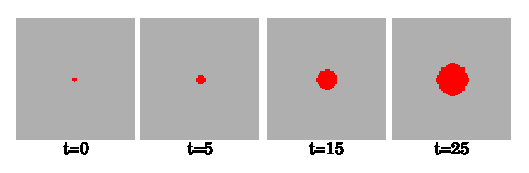
\includegraphics[width=\textwidth]{urban-growt-transitions-1}
      \caption{Růst města bez dalších dodatečných podmínek} 
    \end{subfigure}
    \\
    \begin{subfigure}[t]{\textwidth} \centering
      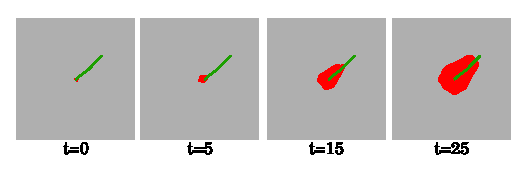
\includegraphics[width=\textwidth]{urban-growt-transitions-2}
      \caption{Růst města podél silnice} 
    \end{subfigure}
    \\
    \begin{subfigure}[t]{\textwidth} \centering
      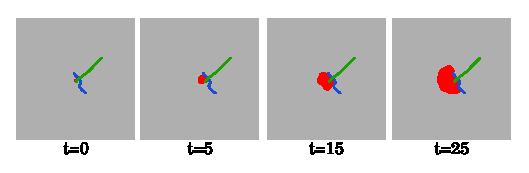
\includegraphics[width=\textwidth]{urban-growt-transitions-3}
      \caption{Růst města bržděn řekou} 
    \end{subfigure}

    \caption[Ukázky chování automatu]{(převzato z \cite{LiuPhi-DevCelAutModUrbGroIncFuzSetApp}) Ukázky chování automatu při různých počátečních konfiguracích. Šedě jsou znázorněny prázdné parcely, červeně zástavba, zeleně hlavní silnice a modře řeky.} \label{img-VarTransRuls}
\end{figure}

Na obrázku \ref{img-UrbGroProSample} je k vidění konkrétní ukázka městského růstu. Na obrázku jsou pro porovnání zobrazeny jak vypočtené stavy zástavby, tak i skutečné (upravené satelitní snímky). Na snímcích je patrné, že simulace rozvoje mezi lety 1987 a 1997 dosáhla poměrně přesných výsledků. Stejně tak, v simulaci růstu mezi lety 1997 a 2005 naznačuje jen malý rozvoj. Při simulaci od roku 1987 do roku 2005 už jsou patrné větší odlišnosti (simulace nevyprodukovala tak výrazný růst, jaký doopravdy nastal).

\begin{figure}[]
    \begin{subfigure}[t]{\textwidth} \centering
      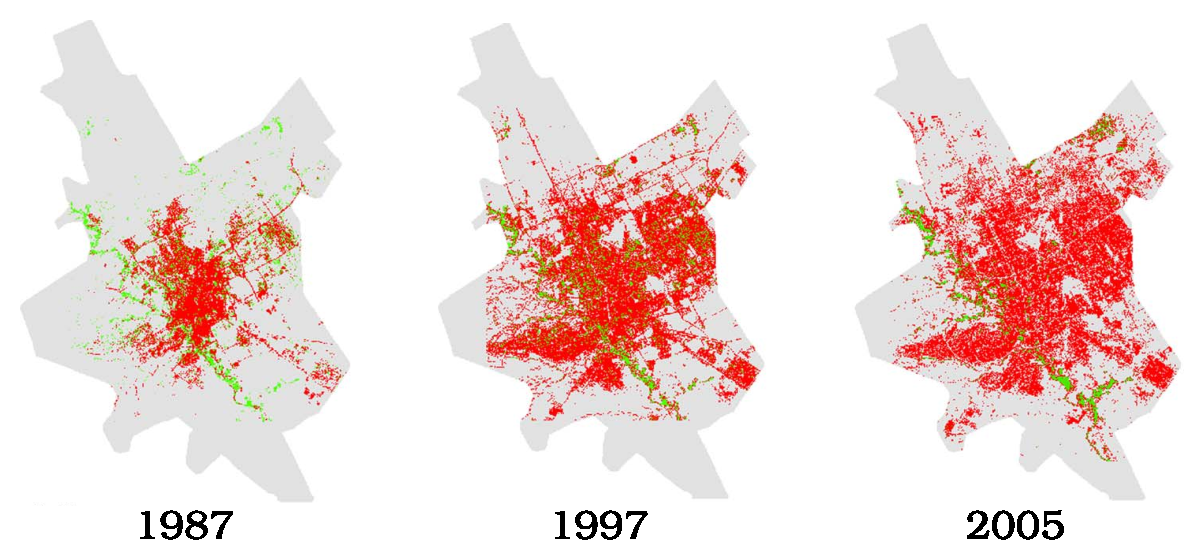
\includegraphics[width=\textwidth]{urban-growt-city-1}
      \caption{Skutečný stav zástavby v uvedeném roce. Červená značí zástavbu, zelená přírodní oblasti (např. vodní plochy) a šedá nezastavěné plochy.} 
    \end{subfigure}
    \\
    \begin{subfigure}[t]{\textwidth} \centering
      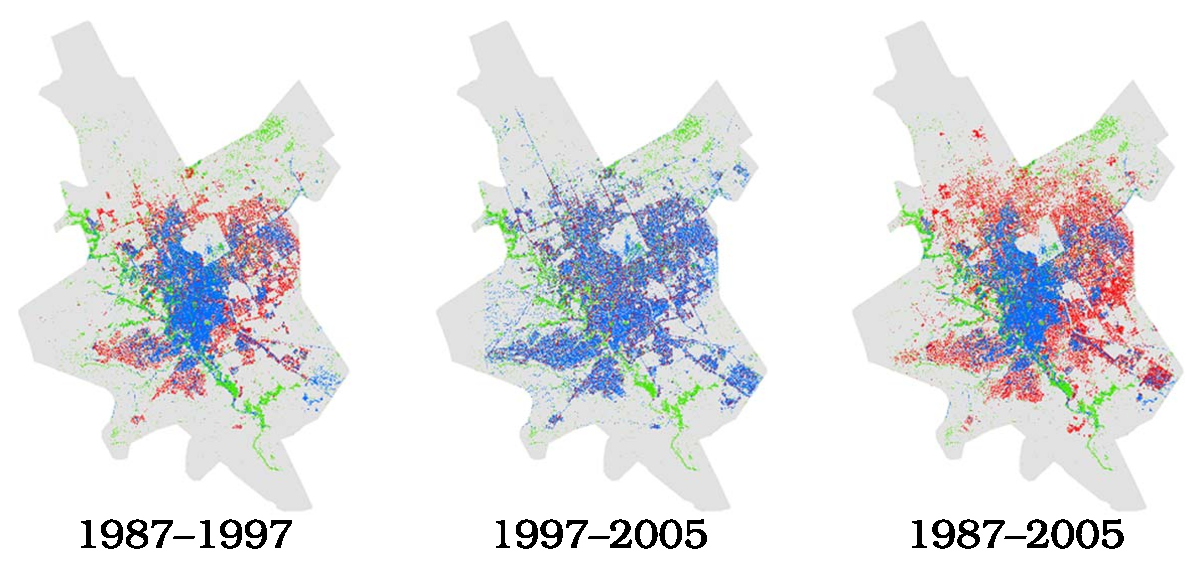
\includegraphics[width=\textwidth]{urban-growt-city-2}
      \caption{Simulovaný stav zástavby. Modrá značí zástavbu na počátku sledovaného období, červená značí (novou) zástavbu na konci sledovaného období, zelená přírodní oblasti (např. vodní plochy) a šedá nezastavěné plochy.} 
    \end{subfigure}

    \caption[Ukázky simulace městského růstu]{(převzato z \cite{Ahm+-CalFuzCelAutModUrbDynSauAr}) Ukázky simulace městského růstu} \label{img-UrbGroProSample}
\end{figure}

Je potřeba zdůraznit, že obyčejná sada přechodových pravidel bývá silně nedostačující. Pro obdržení optimálního výsledku je nutné přechodová pravidla rozšířit o další, sotisfikovanější nástroj nebo nástroje. V praxi se tak nejvíce používají umělé neuronové sítě \cite{LiYe-NeuNetBasCelAutSim+}, \cite{YehLi-SimLanDevIntCelAutMulCriEv}, genetické algoritmy \cite{Ahm+-CalFuzCelAutModUrbDynSauAr}, často však jejich kombinace. V \cite{Dra-CouFuzSetTheGisBaCelAutLanUseChaMod} používají algoritmus fuzzy $k$-means pro určení okolních buněk pomocí shlukování. Návrh automatu tak vyžaduje značné množství experimentů a konzultací s expertem.

%%%%%%%%%%%%%%%%%%%%%%%%%%%%%%%%%%%%%%%%%%%%%%%%%%%%%%%%%%%%%%%%%%%%%%%%%%%%%%%
\subsection{Hledání hran obrázku}
Hledání hran je jednou ze základních technik zpracování obrazu. Rozpoznávání hran je například klíčové pro rozpoznávání vzorů v obrazech. V dnešní době existuje velké množství algoritmů, pro nalezení hran.\TODO{najít nějaký článek je porovnávající} Použití fuzzy buněcných automatů však přichází s elegantním řešením problému. 


Zaostřování obrázku: \cite{MarMeySol-HybMetGasDifModFuzCelAutImSha}, resp. \cite{ZhaLiZha-EdgDetImaBasFuzCelAut} (tam to je vylepšeno pro zašumné obrázky).

\subsection{Další povídání}




\cite{For-FuzCelAutConjNormForm} kóduje stavy sousedů do řetězce $0$ a $1$ (pro každého souseda 1 symbol). Přechodová funkce každé buňky je pak vlastně zobrazení z $\{ 0, 1 \}^m$ do $\{0, 1\}$. Tudíž, $\{ 0, 1 \}^m$ je vstupní abeceda a  $\{0, 1\}$ množina stavů KDA.

Generování růstu krystalů (sněhových vloček, super) \cite{Wol-NewKinSci}.


The Density Classification or Majority problem (poblém hledání shluků)? Simulování kapání vody na haldinu.


For example, CA approaches have been applied in the
context of geocomplexity to earthquakes (Rundle et al. 2000, Weatherley et al. 2000),
lava flows (Crisci et al. 2008, Rongo et al. 2008), density currents (Salles et al. 2007),
surface water flows (Thomas and Nicholas 2002, Doeschl-Wilson and Ashmore
2005, Coppola et al. 2007, Parsons and Fonstad 2007), flooding (Dalponte et al.
2007) (píšou v LaiDraSch-IntMulEvCelAutMetLanSimMod).

%%%%%%%%%%%%%%%%%%%%%%%%%%%%%%%%%%%%%%%%%%%%%%%%%%%%%%%%%%%%%%%%%%%%%%%%%%%%%%%
%%%%%%%%%%%%%%%%%%%%%%%%%%%%%%%%%%%%%%%%%%%%%%%%%%%%%%%%%%%%%%%%%%%%%%%%%%%%%%%
%%%%%%%%%%%%%%%%%%%%%%%%%%%%%%%%%%%%%%%%%%%%%%%%%%%%%%%%%%%%%%%%%%%%%%%%%%%%%%%

\newpage

\section{Konkrétní příklady}
\subsection{Rozpoznávní ručně psaného textu}
...

\subsection{Detekce překlepů}
\cite{AndAbdAsm-ApprPattMatcFuzzLog} až na konci,  Fuzzy Aho-Corasick algorithm (popř. dohledat jiný zdroj).
%%%%%%%%%%%%%%%%%%%%%%%%%%%%%%%%%%%%%%%%%%%%%%%%%%%%%%%%%%%%%%%%%%%%%%%%%%%%%%%
\newpage
\bibliography{resources}
\bibliographystyle{plain}


\end{document}
